
\documentclass[english,letterpaper,12pt]{article}

\usepackage[a4paper,left=2.8575cm,right=2.8575cm,top=2.8575cm,bottom=2.8575cm]{geometry}
\usepackage{lscape}
\usepackage{enumitem}
\usepackage{tikz}


\usepackage{comment}
\usepackage{pdflscape}  


\usepackage{dirtytalk}

\usepackage{placeins}


\definecolor{mygreen}{RGB}{117,167,117}
\definecolor{myred}{RGB}{255,1,1}



\usepackage[utf8]{inputenc}
\usepackage{graphicx, color}

\usepackage{csquotes}


\usepackage{amsmath,amsthm,amssymb}
\DeclareMathOperator*{\argmax}{arg\,max}
\DeclareMathOperator*{\argmin}{arg\,min}
\newtheorem{definition}{Definition}
\newtheorem{assumptionE}{Assumption}

\usepackage{afterpage}
\usepackage{rotating}
\usepackage{setspace}
\usepackage{booktabs,threeparttable,tabularx,ltxtable,longtable,tabu,float,dcolumn,eurosym,lscape,authblk,setspace}
\usepackage[font=footnotesize]{caption}
\usepackage[font=footnotesize]{subcaption}
\usepackage{tabularx}
\usepackage{varwidth}
\usepackage{pdflscape}
\usepackage{framed}
\usepackage[multiple]{footmisc}
\newcolumntype{d}{D{.}{.}{2.5}}
\newcolumntype{s}{D{.}{.}{1.2}}
\newcolumntype{Y}{>{\centering\arraybackslash}X}
\newcolumntype{y}[1]{>{\raggedright\arraybackslash\hsize=#1\hsize}X}
\newcommand\independent{\protect\mathpalette{\protect\independenT}{\perp}}
\def\independenT#1#2{\mathrel{\rlap{$#1#2$}\mkern2mu{#1#2}}}
\usepackage[comma,authoryear]{natbib}
\widowpenalty=15000
\clubpenalty=15000
\bibpunct{(}{)}{;}{a}{,}{,}

\usepackage[pdfborder={0 0 0}, linkcolor=black, urlcolor=blue, citecolor=blue, colorlinks=true,hyperfootnotes=false]{hyperref}

\usepackage{amsthm}
\usepackage{array,multirow}

\newtheorem*{remark}{Remark}
\newtheorem{proposition}{Proposition}
\newtheorem{lemma}{Lemma}

\usepackage{xr}

\newcommand\norm[1]{\left\lVert#1\right\rVert}



\begin{document}

\title{Peer Effects and Rank Concerns in the Classroom} 
\author{ Michela M. Tincani\thanks{ I would like to thank Orazio Attanasio, Richard Blundell, Martin Cripps, Mariacristina De Nardi, Steven Durlauf, Ed Hopkins, \'{A}ureo de Paula, Imran Rasul, Bryony Reich, Elie Tamer, Petra Todd, and participants at various seminars and conferences for insightful comments. Julia Schmieder provided excellent research assistance. Research funding from the Centre for Microdata Methods and Practice and from the European Research Council's grant number IHKDC-249612 is gratefully acknowledged. I am grateful to the Chilean Ministry of Education, the Chilean National Institute for Statistics, and the {\itshape Agencia de Calidad de la Educaci\'{o}n} for access to the data used in this research. }}
	\affil{\small University College London, CEPR, CESifo, HCEO, IFS and LEAP}
	


\maketitle


\begin{abstract}


 I examine how disruptions to students' environments propagate to their classmates to understand the mechanisms behind peer interactions in the classroom. I combine administrative and survey data from Chile with detailed measures of housing damages from the 2010 earthquake, one of the most violent ever recorded. Damages to a student's own home reduced achievement and raised self-reported cost of study effort. Average damages among classmates induced schools to reallocate resources towards student support and increased achievement. In contrast, dispersion in classmates' damages had heterogeneous achievement effects across the prior performance distribution, which schools did not appear to mitigate, pointing to peer interactions. Motivated by evidence suggesting students value classroom rank, I show that a game-of-status model of competition for grades rationalizes the findings. The results suggest that, beyond production complementarities and a desire to conform, a desire to compete could shape peer effects on learning.
 


\end{abstract}

\begin{onehalfspacing}
		
		
		

\section{Introduction}

Childhood and early adulthood are fundamental years for cognitive development (\cite*{cunha2006interpreting}). School peers can affect cognitive achievement during these crucial years\footnote{See \cite*{ammermueller2009peer,arcidiacono2012estimating,booij2017ability,carrell2013natural,duflo2011peer,garlick2018academic,hanushek2003does,hoxby2000peer,imberman2012katrina,lyle2009effects,sacerdote2001peer}.}, but the mechanisms are not fully understood, limiting our ability to design policies that can be effective across contexts. \par 
This paper studies why classroom peers can shape the academic achievement of students. It introduces a new dataset that links students' academic outcomes, self-reported cost of study effort, teacher curriculum coverage, and schools' resource allocation to newly constructed measures of disruptions to students' environment stemming from one of the most violent earthquakes ever recorded. The dataset allows me to study how study disruptions spill over to classmates. Identification relies on variation in peer disruptions rather than in peer characteristics, avoiding confounding effects associated with the latter.\footnote{Examples of studies using naturally occurring exogenous variation in peer characteristics to account for confounding effects are \cite{hoxby2000peer, angrist2004does,hoxby2005taking,lavy2012inside,imberman2012katrina}.} I draw on the empirical evidence to propose a new theory of peer influence in cognitive development. While formulated within the context of an environmental shock, the theory offers a framework to understand why peers matters for learning in many contexts.\par 



The empirical context is the 2010 Maule mega-earthquake, the seventh strongest ever instrumentally recorded \citep{USGSCatalog2025}. I combine administrative and survey data with information on damage propagation among over 150,000 students. I start by building a measure of each student's home's vulnerability to the earthquake using information on housing quality. From the last pre-earthquake census I obtain information on the construction materials of the homes of the nearly one million Chilean households with at least one school-aged child. I employ an unsupervised learning algorithm to stochastically assign their homes to seismic resistance classes. Armed with this housing quality measure, I develop a model that can accurately predict housing quality from a household's characteristics, and apply it to administrative data on Chilean students to predict the quality of their homes. Drawing upon the structural engineering literature, I then combine this newly developed measure of housing quality with geocoded information on ground-shaking intensity in each student's hometown to construct a measure of home damages for each student.\footnote{I gratefully acknowledge Prof. Sergio Ruiz of the Geology Department at the University of Chile, a leading expert on the seismic vulnerability of Chilean buildings, for feedback on the damage measure. The measure falls within Deterministic Earthquake Loss Estimation, which aims to estimate losses from a specific seismic event. It stands in contrast to Probabilistic Earthquake Loss Estimation, which aims to predict potential losses from many possible seismic events (\cite{McGuire2004Seismic}).} This variable measures the shock to each student's environment.\par



I link the damage measure to administrative and survey data from the Chilean Ministry of Education. Data on students include standardized test scores and GPA at two points in time (in fourth and eighth grade), family background, type of school attended, and survey information on self-reported cost of study effort and ability to engage with course content. Data on teachers include the fraction of the curriculum they were able to cover. For the 42\% of schools participating in the preferential school subsidy program (SEP, {\itshape Subvenci\'{o}n Escolar Preferencial}), data include detailed reports on SEP resource spending.  All observations can be assigned to classrooms and schools through unique identifiers.\par  


Using this newly constructed dataset, I first document new facts about socioeconomic segregation among Chilean children. Poorer students were more likely to live in the rural localities experiencing more ground shaking, and conditional on locality, their homes were built according to worse construction standards. As a result, compared with students whose parents have more than 14 years of education (who likely attended some college), those whose parents have at most 14 incurred twice the amount of home damages (USD 1,552 vs. USD 759, or 47\% vs. 23\% of annual household income). \par 

I then estimate the causal impacts on students' outcomes of damages to their own homes and to the homes of their classmates, focusing on the mean and standard deviation of damages among classmates. The identification strategy relies on a difference-in-differences framework leveraging the different correlation between seismic vulnerability and outcomes across two cohorts of students, one whose outcomes were measured in 2009, before the earthquake struck, and one whose outcomes were measured in 2011, after the earthquake struck. This strategy eliminates confounding effects that could arise if the measures of earthquake vulnerability correlated with unobserved outcome determinants. The identifying assumption is that the relationship between outcomes and earthquake vulnerability would be the same across cohorts absent the earthquake. I provide several pieces of evidence supporting this assumption, showing no evidence that students reallocated to classrooms and schools in response to the earthquake in the estimation sample (which excludes by design forced re-locations), showing no impacts on placebo outcomes pre-determined at the time of the earthquake, and showing that the seismic vulnerability of peers' homes does not correlate differently with outcomes across cohorts in regions that were never affected by the earthquake.\par 

Using this strategy, I find that the damage incurred by a student's own home had a negative and non-negligible effect on achievement 22 months post-earthquake. A 1 standard deviation increase in damages lowered test scores by 0.03 standard deviations, and GPA by 0.02 standard deviations, albeit the GPA impacts are statistically insignificant. Using survey data, I provide evidence that damages at the students' own homes increased students' reported cost of study effort, suggesting it could have mediated the detrimental impacts on achievement. \par
Regarding the spillover effect of damages to peers' homes keeping fixed a student's own exposure to the earthquake, I find that increasing the average damages suffered by classroom peers increases own test scores, and the effects are not significantly different across students with different initial performance. This appears to be the result of schools overcompensating any potential negative impacts. Data on school spending show that schools responded to the average level of damages suffered by their students by reallocating resources from recruitment costs toward activities directly linked to student support and learning recovery, such as educational and psychological support.\par 
In contrast, increases in the within-classroom standard deviation of damages lowered the achievement of students with high initial performance and increased the achievement of those with low initial performance. Neither the data on curriculum coverage nor the data on school spending provide statistically significant evidence of schools reacting to how dispersed the damages were, such as by focusing existing resources towards activities targeted at students with lower initial performance. Additionally, emergency funds were granted to schools depending on the overall damage severity, not its dispersion (\cite{Gobierno2010}, Appendix \ref{sec:reconstructionplan}). \par 
The results so far suggest that study disruptions had spillover effects on classroom peers, and that schools mediated the effects of average damages but possibly not of damage dispersion, suggesting a potential role for peer-to-peer interactions. To better understand the damage-dispersion spillovers, I analyze impacts on GPA rank, to examine if the heterogeneous effects on GPA triggered changes to students' GPA rankings in the classroom. Surprisingly, I find this did not occur. Students with higher initial performance experienced drops in GPA in classrooms with more dispersed damages, without an accompanying drop in their GPA rank.  A possible reason for this is that students care about their GPA rank. Faced with a changed cost of study effort among their peers, students adjusted their effort and learning (a peer effect), but not at the expense of their classroom standing in terms of an achievement measure observable to classmates. Rank concerns, therefore, could be a mode of peer-to-peer interactions.\par

 
 

Drawing on this insight and on the empirical findings, I formulate a new theory of interactions in the classroom. I formalize the simple intuition that students care about their classroom standing through a game-of-status model of simultaneous effort choices in the classroom. In the model, students are characterized by an effort-cost type, which is affected by prior test scores, socioeconomic characteristics, and by the damages to their home. They produce GPA by exerting costly effort, and derive utility from GPA and GPA rank. To account for the evidence on schools' reactions, mitigating actions by schools in response to average damages are allowed to enter the achievement production technology. I show that the model, which admits a unique symmetric Bayesian Nash equilibrium, can rationalize the empirical findings. Specifically, a school's mitigating efforts lead to positive effects of average damages. The competition motive behind students' effort choices causes the damage dispersion to have heterogeneous impacts on GPA, and null effects on GPA rank, along the prior test score distribution, conditional on a student's own damage and socioeconomic characteristics. By changing the density of types differently across the effort–cost type distribution, damage dispersion affects incentives differently for different students, both by changing how many nearby types can be overtaken with a marginal increase in effort, and by shifting equilibrium effort responses throughout the distribution. These forces generate heterogeneous effects on the returns to effort and, in turn, on GPA, that are consistent with the patterns found in the data.\footnote{A small strand of the literature on college admissions has developed tournament models of student effort under rank incentives (\cite{bodoh2017pre,grau2018impact,tincani2025college}). These papers study the effects of {\itshape changing} the rank incentives, holding peer characteristics fixed, rather than peer effects {\itshape given} rank concerns. The most relevant is \cite{tincani2025college}: after showing experimentally that rank incentives affect study effort in Chilean high schools, the authors develop and structurally estimate a tournament model of simultaneous effort choices, in which college seats are assigned according to within-school GPA rank.\label{fn:tournaments} }  \par 

The central theoretical insight can be applied more broadly outside the realm of environmental shocks: when competitive motives drive study effort, changing the dispersion of peers' cost-of-effort types, be it through shocks to the cost of effort or through compositional changes from classroom assignment policies, affects learning, and does so differently for different students depending on how the change affects the number of nearby competitors and the effort of all competitors. This has important and so far mostly unexplored implications for policy, as I discuss in this article's concluding section.\par 


Methodologically, this study relates to the small literature that examines peer interactions relying on random shocks to students that keep group composition constant (see the survey in \cite{bramoulle2020peer}). One of the closest studies is \cite{fruehwirth2013identifying}, who exploits the introduction of a student accountability policy in North Carolina targeted at low-achievers. The policy serves as a shock to the effort of some but not all students in the classroom; the fraction of affected peers is used to estimate the impact of peers' achievement on own achievement within a linear-in-means framework.\footnote{\cite{berlinski2023helping} have applied a similar strategy to data from a literacy remediation program in Colombia, and \cite{dieye2014accounting} to data from a randomized experiment on a scholarship program in Colombia. See also \cite{fruehwirth2014can} for an in-depth analysis of the identification of the effect of contemporaneous peer outcomes on own outcomes when outcomes are partly determined by unobserved factors.  } The estimates are interpreted as best-response functions through the lens of a model of effort choices in a strategic environment where students desire to conform to each other. In contrast, this paper considers a continuous shock, the extent of damages that each student's home incurred. Rather than identifying best-response functions, an `endogenous peer effect' in the terminology of \cite{manski1993identification}, this paper examines the reduced-form impact of changing the distribution of the shocks within the classroom, an `exogenous peer effect' in this terminology. Through the lens of a model where students desire to compete with each other, it interprets the estimates as comparative statics on equilibrium outcomes in the classroom.\footnote{Unlike \cite{fruehwirth2013identifying}, I do not estimate the `endogenous peer effect', because the theoretical model does not yield a closed-form expression for the best-response function. Instead, the model characterizes the equilibrium effort function within each classroom, which traces effort as a function of a student's effort-cost type, and derives comparative statics on this equilibrium effort function under different within-classroom distributions for the effort-cost types. When damages to a student's home affect the student's effort-cost type, the model provides testable implications on the shape of the spillovers from earthquake-induced disruptions.} The impacts of the mean and of the dispersion of this continuous shock among peers are shown to be helpful to inform a new theory of peer influence.\footnote{\cite{de2013understanding} also test theories of peer influence. They use evidence on the effects of changing peer composition, which is deliberately kept constant here.}\par 

Within the vast literature on peer effects in education, relatively few studies have developed theories of peer influence. Existing theories commonly assume that students have a desire to conform to their peers, or that there are complementarities between peers in the achievement production technology (e.g. \cite*{brock2001discrete,durlauf2006multinomial,calvo2009peer,fruehwirth2013identifying,conley2024social}). Both assumptions rationalize the workhorse linear-in-means model of peer effects with continuous outcomes (\cite*{blume2015linear}). In contrast, I present a new theory that rationalizes why moments beyond the mean may matter, in a parsimonious way. It offers a simple insight: when students derive utility from rank, changing the cost of study effort of peers affects own effort, because it changes the ability of peers to compete. Empirically, this generates a peer effect where moments beyond the mean matter, without the need to introduce extensions to the technology or preferences to capture the influence of higher-order moments. Such a mechanism has been largely ignored despite its intuitive appeal.\footnote{In line with the theory first introduced in this paper (as detailed in e.g. \cite{tincani2017heterogeneous}), \cite{rosenzweig2023classroom} recently provided evidence supporting this mode of interaction within the context of Southeast Asian refugee students in the US.} \par 
 
The idea that students may care about their rank is consistent with a growing body of evidence showing that competitive preferences can emerge early in life (\cite{sutter2015gender,page2017older}) and that classroom rank can yield both immediate and longer-term benefits. A large literature on {\itshape rank effects} has examined how exogenous changes in a student’s achievement rank within a reference group affect student outcomes. A higher rank has been shown to improve self-concept, happiness, and teacher perceptions of ability, and to raise later educational attainment and earnings (e.g. \cite{zeidner1999big,marsh2007big,elsner2017big,elsner2018rank,murphy2020top,denning2023class,ladant2024essential,carneiro2025effect}). Students, therefore, may value their relative standing, even when it is not formally rewarded. Building on this insight, this paper studies instead the implications of {\itshape rank concerns}, i.e., of students caring about their rank, for how peers influence each other's learning.\par  


This paper also relates to the empirical literature using natural disasters to identify peer effects in education, such as \cite{cipollone2007social}, \cite{sacerdote2008saints}, and \cite{ imberman2012katrina}. In contrast to these studies, it does not use forced relocations of students for identification, focusing instead on variation in the intensity of disruptions.\footnote{This distinguishes this paper also from the experimental and quasi-experimental literature that use variation in assignment to peer groups, such as dorms (\cite{sacerdote2001peer,zimmerman2003peer,Stinebrickner2006,kremer2008peer,garlick2018academic}) or classrooms (\cite{duflo2011peer,whitmore2005resource,kang2007classroom}).} I interpret these disruptions as shocks to a primitive of the students' skill-accumulation problem that shape their effort choices. This interpretation, consistent with the skill-formation framework where human capital reflects optimally chosen investments (\cite{todd2003specification,cunha2008formulating,cunha2010estimating}), allows me to move beyond measuring earthquake spillovers to shed light on how social interactions influence those investment decisions. Finally, the paper relates to the empirical literature on ability peer effects studying the impacts of moments beyond the mean (\cite{lyle2009effects,booij2017ability,ding2007peers,vigdor2007peer, hoxby2005taking}) and of partitioning the support of ability, which varies first and higher-order moments simultaneously (\cite{carrell2013natural,duflo2011peer}). These studies tend to find that moments beyond the mean matter for learning. \par 




The article is structured as follows. Section \ref{sec:data_and_measurements} details the data, damage measure, and describes damage propagation among students, documenting new facts about socioeconomic inequalities. Section  \ref{sec:analysis_earthquake_effects} delves into the empirical analysis of damage effects on achievement, and assesses the identifying assumption and robustness. Section \ref{sec:mechanisms} presents evidence on mediating factors using administrative and survey data. Section \ref{sec:new_theory_peer_effects} introduces the theory of peer influence based on rank concerns, rationalizing the evidence. Section \ref{sec:conclusions} concludes, discussing policy implications and suggesting future research avenues. \par 
	
\section{Data and Measurements}\label{sec:data_and_measurements}
This section describes the data sources and measurements and performs a descriptive data analysis.
\subsection{Data}\label{sec:data}
I construct a dataset on two cohorts of students combining information from the SIMCE datasets  ({\itshape Sistema de Medici\'{o}n de la Calidad de la Educaci\'{o}n}, \cite{agencia_simce_scores}) and enrollment and grade registries ({\itshape Rendimiento} and {\itshape Matr\'{i}cula}, \cite{mineduc_rendimiento_2005_2010,mineduc_matricula_2009}). I refer to the two cohorts as pre- and post-earthquake cohorts, depending on whether their outcomes were measured before or after the earthquake. The $8^{th}$ grade outcome for the pre-earthquake cohort is observed in 2009, before the 2010 earthquake, the $8^{th}$ grade outcome for the post-earthquake cohort is observed in 2011, 20 to 22 months after the 2010 earthquake (Figure ~\ref{data_timeline}). The sample includes students in public and private subsidized schools.\footnote{I exclude students from the elite private unsubsidized schools. They represent approximately $7\%$ of the student population and they come from the most well-off families in the country.} I obtained from the Ministry of Education the list of schools that closed as a consequence of the earthquake, and used registry data to identify the schools where the evacuated students relocated to (\cite{tincani_school_closures}). I dropped from the sample both sets of schools, from both cohorts, to ensure the absence of earthquake-induced relocations in my sample.\footnote{I dropped $36,941$ observations from the post-earthquake cohort and $38,784$ from the pre-earthquake cohort, corresponding to $13\%$ of the sample.} Such relocations could directly affect the outcomes of evacuated students and indirectly those of incumbent students in receiving schools through changes in peer composition. Such effects could confound the effects of interest in this paper. I dropped observations with missing classroom identifiers,\footnote{These are $17,944$ observations in the post-earthquake cohort and $21,194$ observations in the pre-earthquake cohort. The school and student identifiers are never missing.} and classrooms with five or fewer students.\footnote{These correspond to $2,484$ student-level observations, or $0.7$ percent of the sample.} The full constructed dataset consists of $354,133$ students in $13,268$ classrooms across $8,974$ schools. The main estimation sample is restricted to students living in regions affected by the earthquake; students living in non-affected regions are used only for testing the identifying assumption. As explained in the next section, to mitigate measurement error in the damage measure the main analyses exclude around 15\% of observations, corresponding to schools located in coastal towns. Table \ref{summaryprepost} reports the sizes of the pre- and post-earthquake cohorts under each restriction.   \par  

 For both cohorts I observe administrative records on $8^{th}$ grade and $4^{th}$ grade Mathematics and Language standardized test scores and school grades, gender, town of residence and unique student, classroom and school identifiers. I complement these data with linked survey data on students' perceptions (\cite{agencia_simce_student_questionnaire}), and on the household socioeconomic background (\cite{agencia_simce_parent_questionnaire}). Administrative school-level information includes rurality and public or private status. I complement this information with teacher surveys on curriculum coverage (\cite{agencia_simce_teacher_questionnaire}) and, for a subset of schools, with detailed reports on school expenditures (\cite{mineduc_sep_expenditure}). Finally, I match students to classrooms, teachers and schools through unique pseudo-identifiers.
\begin{figure}
	\centering
	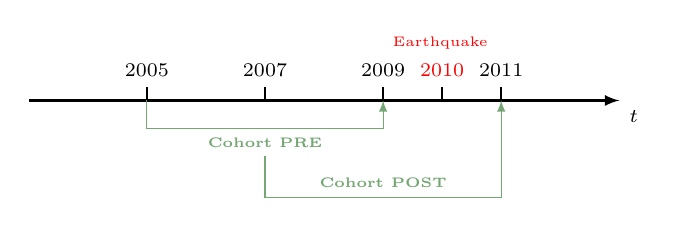
\begin{tikzpicture}[x=1.5cm]
		\draw[black,->,thick,>=latex]
		(0,0) -- (5,0) node[below right] {$\scriptstyle t$};
		
		
		\draw[black,thick]
		(1,0) -- ++(0,5pt) node[above] {$\scriptstyle 2005$}
		(2,0) -- ++(0,5pt) node[above] {$\scriptstyle 2007$}
		(3,0) -- ++(0,5pt) node[above] {$\scriptstyle 2009$}
		(3.5,0) -- ++(0,5pt) node[above,color=myred] {$\scriptstyle 2010$}
		(4,0) -- ++(0,5pt) node[above] {$\scriptstyle 2011$};
		
		%Annotations
		\node[above right, color= myred] at (3,15pt) {\tiny Earthquake};
		\node[below, color=mygreen] at (2,-10pt) {\tiny {\bf Cohort PRE}};
		\node[above, color=mygreen] at (3,-35pt) {\tiny {\bf Cohort POST}};
		
		\draw[mygreen, ->,>=latex] (1,0) -- (1,-10pt) -- (3,-10pt) -- (3,0pt) ;
		
		\draw[mygreen, ->, >=latex] (2,-20pt) -- (2,-35pt) -- (4,-35pt) -- (4,0pt) ;
		
	\end{tikzpicture}
	\caption{Data time-line.\label{data_timeline}}
\end{figure}

\subsection{Measuring damages to homes } \label{sec:measure_damages_to_homes}

\paragraph{Earthquake.} On February $27^{th}$ 2010, at 3.34 am local time, Chile was struck by a magnitude 8.8 earthquake, the seventh-largest ever instrumentally recorded and technically referred to as a mega-earthquake (\cite{astroza2012}, \cite{USGSCatalog2025}). Figure \ref{fig:earthquake_distribution} shows its position in the global earthquake distribution since 1900. Shaking was felt strongly throughout 500 km along the country, covering six regions that together make up approximately $80\%$ of the country's population. Damage was widespread, with costs estimated at 18 percent of GDP (\cite{oms2010terremoto}). The Government implemented a national plan to rebuild or repair housing units for low- and middle-income families. The mega-earthquake had continued impact on people's lives during the period covered by my sample. The post-earthquake cohort, whose outcomes were collected when they were in the $8^{th}$ grade in 2011, was about to start the $7^{th}$ grade when the earthquake struck. By the time the 2011 outcome data were collected, 20-22 months had passed since the earthquake struck. Yet, only 24 percent of home reconstructions and repairs had been completed (\cite{comerio2013housing}), leading to frustration in the population (Appendix Figure ~\ref{fig:dios}). 




\begin{figure}[h!] 
 	\centering
 	\includegraphics[scale=0.65]{output/figures/earthquake_distribution.png}
 	\caption{{\itshape Source}: Global Earthquake Catalog maintained by the United States Geological Survey (\cite{usgs_earthquake_catalog}). }
 	\label{fig:earthquake_distribution}
 \end{figure}







\paragraph{Measuring earthquake damage to a student's home.} The damage to a student's home depends on the level of ground shaking and on the construction materials. I proceed in three steps. First, I construct a measure of the shaking that each student's home was subject to. Second, I build a measure of the seismic vulnerability of each student's home, which depends on the construction materials. Third, I combine these two measures to calculate home damages. I now describe each step.\par  

 \paragraph{Step one: ground shaking.} For students who reside in earthquake-afflicted regions, I build a measure of distance between each student's town of residence and the asperity centroid as $\Delta_A=\sqrt{R^2+h^2}$, where $R$ is the distance between the town's center and the point on the earth's surface vertically above the asperity centroid, whose coordinates are ($34.8^{o}$S, $72.6^{o}$W), and $h=20$km is the depth of the latter (the town-level distances $R$ are from \cite{tincani_distance_measures}). I then apply the intensity attenuation formula derived by \cite{astroza2012} for the 2010 Chilean earthquake that gives for each distance $\Delta_A$ a level of severity of ground shaking, $I$, measured on the Medvedev-Sponheuer-Karnik (MSK) scale: $I=19.781-5.927\log_{10}(\Delta_A)+0.00089\Delta_A$ ($R^2=0.9894$).\footnote{$\Delta_A$ is non-negative because it measures a distance, and it is never equal to zero because no town was directly above the asperity, which was in the ocean. The reported $R^2$ refers to the reported regression with MSK-Intensity as outcome variable. }\par 
 

\paragraph{Step two: seismic vulnerability.} A building's seismic vulnerability depends on its construction materials. The construction materials of students' homes are not included in the education dataset, but they are included in census data. Therefore, I use census data to develop a model that can accurately predict the seismic vulnerability of a household's home from a set of observable household characteristics that are available in the education dataset, and I apply this model to the education dataset to build a measure of the seismic vulnerability of the homes of the students in my sample. The procedure comprises three steps. In the first, using census data I build a measure of seismic vulnerability of a building based on its construction materials. In the second, using census data I develop the prediction model and assess its ability to correctly predict housing quality from household characteristics. Finally, I apply the prediction model to the students in my sample (the education data). I now describe the first two steps in more detail (the third step is trivial).  \par 


 

The first step consists in building a measure of seismic vulnerability of a home from information on its building materials as per census data. I obtained the 2002 census data, the last one before the earthquake struck, from the Chilean National Institute for Statistics (\cite{ine_censo_2002}). I restricted the data to the nearly one million households with at least one school-aged child, and extracted information on the construction materials of their homes: for the exterior walls, roof and floor. Table \ref{distrib_materials} in the Appendix shows the distribution of building materials in this population.\par 
 I then mapped the vector of building materials into a predicted seismic vulnerability class (\cite{grunthal1998european}, Table 1). To do so, I estimated a logistic latent-class-analysis (LCA) model that assigns to each home the predicted probabilities of belonging to each of three classes, an unsupervised learning algorithm. Post-estimation, I predicted the distribution of building materials by class. As an unsupervised algorithm, LCA does not label the classes, a step requiring human input. I attached a label to each class (low, medium or high seismic vulnerability) depending on the similarity between the predominant construction materials within each class generated by the LCA model and the predominant construction materials used in Chile within each seismic vulnerability class \citep{massoneintensidades}. In this step of the data construction, I obtained feedback from a leading expert on the seismic vulnerability of Chilean buildings.\footnote{I thank Professor Sergio Ruiz of the Geology Department at the University of Chile for his expert feedback on this step of the data construction, confirming that the distribution of building materials within the classes generated by the algorithm correspond to that found within the seismic vulnerability classes in Chile.}\footnote{\cite{astroza2012} identify four seismic vulnerability classes in Chile, but two of them (confined masonry and confined masonry designed according to the NCh2123 Chilean Code) are indistinguishable from each other using census information. Therefore, I group them into one class. These two types of constructions have the best earthquake resistance profiles (see Table 2 in \cite{astroza2012}), so they are assigned to the low vulnerability class. But in calculating damages, I acknowledge that this class contains two different kinds of constructions: I assume that half of these homes are built according to the NCh2123 Chilean Code, and half are not.} Figure \ref{fig:vc} shows the predicted class proportions in the population of households with at least one school-aged child in the census and the within-class distributions of construction materials.
 
 \begin{figure}[h!] 
 	\centering
 	
\includegraphics[scale=1.3]{output/figures/donut.png} %0.7
 	\caption{Results of the latent-class-analysis model estimated on census data: distribution of seismic vulnerability classes and of building materials within each class (N=929,647). {\itshape Notes}: The percentages next to each class label represent the proportion of homes in that class in the population of households with at least one school-aged child in the 2002 census.}
 	\label{fig:vc}
 \end{figure}

 The second step consists in building a model that can accurately predict the seismic vulnerability of a household's home based on household characteristics, in the population of families with school-aged children. The dependent variable is seismic vulnerability as obtained from the LCA model, that is, a vector containing the probabilities that a home belongs to the low-, medium- or high-vulnerability class. For the independent variables, I restrict attention to the characteristics that are available in both the census and the education data. These are: the age of the household head, the average years of education of mothers and fathers, and the region of residence, to capture any differences in construction standards across regions.\footnote{I assume that the parent who fills out the education questionnaire is the household head.} \par 
  Predicting seismic vulnerability from household characteristics is remarkably easy in Chile, as I find striking socioeconomic stratification in housing quality among Chilean families with school-aged children. As shown in Figure \ref{fig:vc_by_peduc}, students from high socioeconomic status (SES) households are those most likely to live in homes with low seismic vulnerability, students from middle SES households in homes with medium seismic vulnerability, and students from low SES households in homes with high seismic vulnerability. Such socioeconomic segregation is not built into the seismic vulnerability measure, which is constructed only from construction materials. Therefore, the fact that the distribution of seismic vulnerability varies as expected with SES informally validates the procedure I developed to construct seismic vulnerability. To my knowledge, this is the first direct evidence that housing quality, in terms of earthquake resistance, is highly segregated along socioeconomic lines among Chilean students.  \par 
 

 
 

 
 \begin{figure}[!ht] 
 	\centering
 	\includegraphics[scale=0.15] {output/figures/class_prob_by_p_educ_all.png} %0.33
 	\caption{Evidence of socioeconomic segregation in housing quality among Chilean families with school-aged children. This graph plots the probability that the home of a school-aged child belongs to each of three seismic vulnerability classes (low-, medium- and high-vulnerability) by the education of the parents. {\itshape Sources:} census 2002 data, restricted to households with at least one school-aged child (N = 929,647). Class probabilities stem from latent-class-analysis using census information on the construction materials of the families' homes. }
 	\label{fig:vc_by_peduc}
 \end{figure}
 

 
I build the prediction model by estimating a regression on census data. The model can be used to predict the seismic vulnerability of the homes of students in the education dataset because it uses household characteristics available in both the census and the education dataset. Appendix \ref{sec:sv} describes the model. For each household, the model predicts the probabilities that the home belongs to each of the three seismic vulnerability classes. Figure \ref{fig:fit_vc_prediction} shows that its fit is excellent: the housing quality predicted using the estimated model traces very closely the actual housing quality built from information on building materials. The fit worsens slightly only among very old or very highly educated parents, who are very few in the education dataset. This gives me confidence that the model can accurately predict seismic vulnerability for nearly all students in the education dataset. The estimation of the prediction model uses data on the entire Chilean population of families with school-aged children, therefore, it is free of finite-population sampling variability. \par 



 \begin{figure}[!ht] 
	\centering
	\includegraphics[scale=0.18]{output/figures/fit_vc_prediction_all.png} %0.43
	\caption{Goodness of fit of predicted seismic-vulnerability-class probability by parental education and by age of household head. {\itshape Notes:} census 2002, families with school-aged children (N = 929,647). }
	\label{fig:fit_vc_prediction}
\end{figure}





 
 \paragraph{Step three: combining ground shaking and seismic vulnerability to build a measure of damages.} For each student in the sample I now have measures of the intensity of ground shaking and of the seismic vulnerability of her home. I combine these two pieces of information to build a measure of expected damage, defined as the fraction of the home that needs to be rebuilt. The procedure is as follows.\par 
 For each vulnerability class and ground shaking level, \cite{astroza2012} provide the distribution of damage grades, which are divided into six categories, ranging from no damage ($DG=0$) to complete collapse: ($DG=5$). Following \cite{bommer2002development}, I assign to each category $DG_m$ a numerical damage measure $d(DG)\in[0,1]$, called ``damage ratio," which measures damages as a fraction of complete collapse, where $d=1$ represents complete collapse. If the vulnerability class was observed, we could obtain the expected damage ratio of household $i$ given its vulnerability class $vc_i$ and ground shaking intensity level $I_i$ as $E[d_i|vc_i,I_i]=\sum_{m=0}^5 d(DG=m) p^m(vc_i,I_i)$, where $p^m(vc_i,I_i)$ is the probability that a house of vulnerability class $vc_i$ subject to ground shaking $I_i$ suffers a damage grade $DG=m$, which carries a level of damage ratio equal to $d(DG=m)$. But the vulnerability class is not observed. Instead, for each student in the data I observe a vector of predicted probabilities that her house belongs to one of each vulnerability class. Therefore, for each household with characteristics $x_i$ I use the predicted likelihood that it belongs to each vulnerability class $j=1,2,3$ ($\hat{p}^j(x_i)$ in Appendix \ref{sec:sv}) to build a measure of the expected damage ratio:
 
 \begin{equation}\label{eq:measure_damage}
 d_i=E[d|x_i,I_i]=\sum_{j=1}^3 \hat{p}^j(x_i)\cdot \left(\sum_{m=0}^5 d(DG=m)p^m(vc=j,I_i)\right)
 \end{equation}
 
   
 \noindent I standardize this measure in the sample so that it has mean zero and unit variance. This is the measure of home damage used throughout the analysis.\par 

 \paragraph{Tsunami.} The damage ratio is not designed to measure damage stemming from the accompanying tsunami that afflicted coastal towns. In coastal areas it may suffer from larger measurement error, which would lead to attenuation bias. To avoid this, I restrict the sample to non-coastal towns, defined as those located more than 1 km from the coast,  verifying the robustness of the results to different geographical restrictions. This sample restriction excludes approximately $15\%$ of the observations from the analysis.\par 
 
 

 

\subsection{Descriptive analysis}\label{sec:descrptive}


I document new facts about the propagation of damages from the 2010 Maule earthquake among students.\par 

Among students of the post-earthquake cohort who live in earthquake regions (i.e., the students affected by the earthquake), the fraction of the home that collapsed ranged from $0\%$ to $59\%$, and on average was $1.7\%$ (Panel A, Table \ref{tab:descdamages}). The distribution was right-skewed, with most students ($\sim 95\%$) suffering damage ratios below $7\%$. Average reconstruction costs amounted to USD $1,439$, with a standard deviation of USD $3,540$. To express damages relative to households' resources, I also compute the ratio of damage to annual household income. The average of this ratio is 0.43, and its standard deviation is 1.55.\footnote{These back of the envelope calculations use the $2010$ USD to CLP exchange rate, and depend on the assumed cost of reconstructing a completely collapsed home. I assume the cost is equal to the average market price of a $50m^2$ home in Chile in 2010, which was USD $84,175$ (see \url{https://www.globalpropertyguide.com/Latin-America/Chile/square-meter-prices}). If a home suffered an unstandardized damage ratio of $x\%$, then the damage in dollars is measured as $x\% \cdot 84,175$. In the main analyses, I use the standardized damage ratio $d_i$, defined in equation \eqref{eq:measure_damage}, as the measure of damages, because its value does not depend on assumptions on home reconstruction costs.} Lower earning households incurred disproportionately higher damages; a $1\%$ increase in earnings is associated with USD $76$ fewer damages. \par 


We have already seen that students from lower SES live in homes with larger seismic vulnerability (Figure \ref{fig:vc_by_peduc}). Figure \ref{fig:damages_peduc} shows that also the level of home damage, which depends on both seismic vulnerability and ground shaking, decreased with students' SES, as measured by parental education. On average, the homes of students whose parents have at least some college education incurred $793$ fewer USD of damages, or half the amount, than those of students whose parents do not have any college education. The Figure also shows that at all levels of parental education, students in public schools suffered more home damage than those in private schools, and those in rural schools more than those in urban schools. The evidence therefore suggests that the homes of the more disadvantaged students (i.e., those with less educated parents, those in public schools, those in rural schools) suffered the largest earthquake damages. Appendix Table \ref{tab:correlates} shows how all student and school characteristics correlate with home damages and building quality. \par 



\begin{figure}[!ht] 
	\centering
	\includegraphics[scale=0.15]{output/figures/damages_peduc.png}
	\caption{Relationship between home damage and parental education by school characteristics. {\itshape Notes:} sample of students in earthquake-affected regions in the post-earthquake cohort and residing more than 1 km from the coast. The figures present local polynomial regression estimates with $95\%$ confidence intervals. Home damage is measured by the standardized damage ratio $d_i$, defined in equation \eqref{eq:measure_damage}. The top and bottom $1\%$ of observations in terms of parental education were trimmed.}
	\label{fig:damages_peduc}
\end{figure}


Why did homes of disadvantaged students incur greater damage? Figure \ref{fig:damage_propagation_by_SES} visually displays this disparity across two panels, each featuring a map of how damage propagated geographically. The left panel is based on lower-SES students --- those without college-educated parents --- while the right is based on higher-SES students --- those with college educated parents. The circle size indicates the proportion of the respective SES populations living in a particular town. The color intensity indicates the average damage severity for students in that town and SES group, with darker colors indicating worse damage.\par 



\begin{figure}[h!] 
	\centering
	\includegraphics[scale=0.65]{output/figures/damage_propagation_by_SES_py.png}
	\caption{Map of Chile showing propagation of damage from the 2010 Maule earthquake among students by socioeconomic demographics. {\itshape Notes:} The left panel shows damage propagation among students whose parents do not have college education, the right panel among students whose parents have college education. Each circle represents a town. Its size represents the percentage of the sample of non-college-educated parents (left panel) or of college-educated parents (right panel) living in that town. The shade reflects the average level of damages to the homes of the students without (left panel) or with (right panel) college-educated parents in that town,  measured in USD. For reference, the average annual wage in the entire sample is USD 8,378. College education is defined as having more than 14 years of education, as most vocational higher-education degrees require at most 14 years of education. Data source for country boundaries: \cite{natural_earth_admin0}. }
	\label{fig:damage_propagation_by_SES}
\end{figure}




The maps reveal that lower-SES students were more likely to live in the (mostly rural) areas most affected by the earthquake than higher-SES students. But even conditional on residing in the same town, the homes of lower-SES students were more damaged, because of lower-quality housing. Damage propagation, therefore, was unequal across socioeconomic lines in Chile because of differences in residential choice and housing  quality. While such socioeconomic inequality may appear unsurprising, this is one of the first studies to document it. \par 




There is variation in how students in the same classroom were affected by the earthquake: $98\%$ of students from the post-earthquake cohort going to school in affected non-coastal areas were enrolled in classrooms where not all students suffered equal damages. This fraction is nearly the same across public and private schools ($98.0\%$ vs. $97.5\%$), and slightly larger among urban ($97.9\%$) than rural ($95.9\%$) schools. As shown in Panel Aii of Table \ref{tab:descdamages}, students were exposed to substantial dispersion in earthquake damages. The average within-classroom standard deviation of the non-standardized damage ratio (the fraction of the home that collapsed) is $0.5\%$, which corresponds to USD 417 at 2010 reconstruction costs. As an alternative scale, I also compute the damage-to-family-income ratio for each student and the standard deviation of this ratio within each classroom. On average, the standard deviation of this ratio is 37\%, meaning that in a typical classroom, home damages differed across students by about 37\% of households' own annual income. In some classrooms the standard deviation in damages reached staggering levels, such as $6.1\%$  at the $99^{th}$ percentile, or USD $5,132$, over seven months' worth of income. Therefore, while students attending the same classroom tended to live in nearby towns and belong to similar socioeconomic classes, there was variation within classrooms in how students were affected by the earthquake, driven by differences in ground shaking and housing quality. This provides rich within-classroom variation in individual-level shocks.\par 

Variation in damages did not only arise within classrooms, but also across classrooms within the same schools and across schools. Intra-class correlation estimates reveal that $91.0\%$ of the total variance in home damages was explained by differences between schools, with the remaining variation occurring within schools. There was also variation in the classroom-level dispersion in damages: 87.4\% of its total variance occurred across schools, with the remaining variation occurring within schools. By contrast, virtually all the variation in the classroom-level mean in damages was across schools (99.8\%).\par 




Finally, Table \ref{summaryprepost} presents descriptive statistics of the pre- and post-earthquake cohorts of students, both country-wide and for the main estimation sample, which display similar characteristics. The descriptive statistics for individual and classroom-level damage-based variables in both cohorts are reported in Appendix Table \ref{tab:descdamages}.\par  


\input{output/tables/descriptive_pre_post.tex}





\section{Empirical Analysis of Earthquake Effects}\label{sec:analysis_earthquake_effects}



\subsection{Main findings}\label{sec:main_findings}

Damages to students' homes varied based on the quality of their homes and the distance of their hometown from the earthquake's asperity. This suggests that we can estimate the causal impact of earthquake damages on student outcomes by using data from a cohort of students with measurable pre-existing vulnerability to the earthquake but whose outcomes were measured before the earthquake struck. A difference-in-differences estimator exploits the differential correlation between vulnerability and outcomes across cohorts to tease out causal impacts.\footnote{In this section, ``vulnerability" refers to overall vulnerability, measured in damage ratios, which considers both construction quality and distance from the asperity.}\par 


Equation \eqref{regression1} presents the regression model I estimate. I consider two achievement outcomes: GPA, which depends on teachers' grades and is in principle observable to classroom peers, and standardized test scores, which are graded centrally and are not directly observed by peers. I use the damage ratios defined in equation \eqref{eq:measure_damage} to measure pre-existing earthquake vulnerability, which reflects actual home damages only for the cohort exposed to the earthquake. The vector $D_{ic}$ of vulnerability variables comprises the damage ratio of student $i$ and the (leave-one-out) mean and standard deviation of damage ratios in $i$'s classroom $c$. The dummy variable $post_i$ takes on value $1$ if a student belongs to the post-earthquake cohort, the one exposed to the earthquake, and $0$ otherwise. The vector $x_i$ of student characteristics includes a lagged achievement measure (the standardized test score in grade 4). The vector $w_{cs}$ of characteristics of classroom $c$ in school $s$ includes the school building's vulnerability.\footnote{ I do not observe the construction materials of the school building, but I observe the shaking intensity in the school's town. To allow for different shaking-resistance levels depending on construction materials, I include as regressors the shaking in the school's town, the shaking interacted with whether the school is public or private (to account for building quality differences across public and private schools),  the shaking interacted with the cohort dummy, the shaking interacted with both the public school and cohort dummies, and the cohort and public school dummies interacted.} The Table notes contain the full list of regressors. \par 





\begin{equation}\label{regression1}
    y_{ics}=\alpha_0 +\alpha_1\cdot w_{cs} + \alpha_2\cdot  x_i + \beta^{'}\cdot  D_{ic}+  post_i\cdot \left[ \gamma + \delta^{'}\cdot D_{ic}\right] +\epsilon_{ics}.
\end{equation}


 For the pre-earthquake cohort, the parameter $\beta$ captures the spurious relationship between vector $D_{ic}$ and outcomes: the location and quality of a student's and her classmates' homes could correlate with unobserved outcome determinants. If such spurious relationship is constant across cohorts, an assumption I assess in section \ref{sec:testing}, the $\delta$ parameters reveal the effects of earthquake damages on achievement, keeping school building damages fixed. This is the parameter vector of interest. \par 

Table \ref{tab:effectsts} presents the results. The outcome in column (1) is the average between the Mathematics and Language SIMCE standardized test scores in eighth grade. Appendix Table \ref{tab:effectsspanmath} shows that considering the two subjects separately yields similar patterns, with somewhat stronger effects on Language at the point estimates. The outcome in column (2) is the GPA in eighth grade, standardized. A one standard deviation increase in a student's damage ratio, corresponding to increasing the collapsed portion of the home by 4.2 percentage points (around USD $3,500$ in damages), lowers test scores by 0.03 standard deviations (std) and GPA by 0.02 std, albeit insignificantly for GPA. To put the magnitude into perspective, this impact is a fifth of that of a one-standard-deviation improvement in teacher value added (\cite{chetty2014measuring}).\footnote{Teachers are one of the most important school inputs into the production of achievement, but school inputs are generally not as impactful as home interventions (e.g. \cite*{zhou2022impacts}, \cite{heckman2006skill}).}\par 

\input{output/tables/main_effects_ts_GPA}


The average damages to the homes of classmates have positive effects on own test scores and GPA. An increase in mean peer damages of one standard deviation of the damage distribution (i.e., a 4.2 percentage point increase in the portion of the home that collapsed) increased test scores by 0.05 standard deviations, and GPA by 0.04 standard deviations. This suggests that schools counteracted any potential adverse learning conditions caused by average damages. Overcompensation in response to the earthquake was documented also in post-earthquake crime prevention in Chilean municipalities (\cite{hombrados2020lasting}). Classroom-level damage dispersion had negative effects on test scores and GPA, of similar magnitudes. An increase in the within-classroom standard deviation of damages of one standard deviation of the damage distribution (i.e., a 4.2 percentage point increase in the portion of the home that collapsed) lowered test scores and GPA by around 0.085 standard deviations. These results suggest that schools did not entirely compensate detrimental effects on student learning due to damage dispersion within classrooms. \par 


To summarize, damages affected the learning of the student living in the damaged home. The detrimental impacts occurred at a critical time in the educational path of students (the year before transferring to secondary education) and were disproportionately borne by students of lower socioeconomic status due to their greater exposure (Figures \ref{fig:vc_by_peduc} and \ref{fig:damage_propagation_by_SES}). While schools could not mitigate the impact of such individual-level shocks, they appear to have successfully mitigated the effect of the average level of damage in the classrooms. By contrast, dispersion in damages across classmates had negative effects on learning outcomes, on average.\par 


\subsection{Identifying assumption}\label{sec:testing}


  The identifying assumption underlying the estimator is that the relationship between achievement and the earthquake vulnerability variables would be the same in the pre- and post-earthquake cohorts in the absence of the earthquake. A concern is that the estimates may capture changes in this relationship across cohorts, rather than true damage impacts. For example, the estimate of the impact of mean damages in the classroom would be biased if the government introduced a policy between 2009 and 2011, the period between the outcomes for the two cohorts were measured, that changed the student composition across schools, such as changes to the vouchers for disadvantaged students to attend private schools.\footnote{Chile has a voucher policy in place, but it did not undergo any changes at this time (\cite{neilson2021targeted}).} If such a policy were introduced, it could alter how a school's mean damage measure, based on the socioeconomic composition, correlates with its unobserved quality across cohorts. This would violate the identifying assumption. To address such concerns, all specifications include a set of controls for socioeconomic composition. By the same logic, they include controls for individual characteristics.\footnote{Appendix Table \ref{tab:effectstscontrolsyn} shows that effect estimates are slightly larger but broadly similar in specifications without such individual and group controls, retaining only the three individual characteristics used to build the damage measure.} Identification, therefore, relies on variation across students and classrooms in earthquake exposure, keeping fixed student characteristics and classroom characteristics such as socioeconomic status.\par

As the earthquake occurred a few days before the start of grade 7 and outcomes are measured in grade 8, a second concern is that the estimates may capture the effect of a reallocation of students across classrooms and/or schools between grades 7 and 8, occurring in response to earthquake damages, that the strategy above and the exclusion from the sample of forced relocations immediately after the earthquake (Section \ref{sec:data}) fail to account for. To examine this, I tracked the movement of students across schools and classrooms between the $7^{th}$ and $8^{th}$ grades, for both cohorts.\par

Table \ref{tab:descriptiveswitches} reports the descriptive analysis. Switches between the $7^{th}$ and $8^{th}$ grades are not common: only $11\%$ of students in the whole sample changed either school or classroom between these grades. This is aligned with what we would expect: students typically move school one grade later, during the transition from primary to secondary school. The vast majority of switches concern school changes: $8.6\%$ of students changed school, while conditional on staying in the same school, only $2.8\%$ changed classroom. Focusing on students and schools in earthquake regions and residing more than 1 km from the coast, the main sample of analysis, I find similar frequencies of all types of switches, as can be seen in the right panel of Table  \ref{tab:descriptiveswitches}. \par 


Next, I analyze whether students could have moved between the $7^{th}$ and $8^{th}$ grade in response to the earthquake. In the main analysis sample (earthquake regions, non-coastal towns), the fraction of overall switches, school switches, and classroom-within-school switches is identical in the pre- and post-earthquake cohorts, as shown in Panel A of Table \ref{tab:effectsswitch}. This suggests that changes to schools or classroom enrollments between these grades were not a margin of response to the earthquake.\par


\input{output/tables/effects_on_switches}


 To complement the before-after analysis, I implemented a difference-in-differences analysis that examines whether the change in switches across cohorts differed between the regions afflicted and those not afflicted by the earthquake. This additional analysis delivers precise zero effects as well, as can be seen in Panel B of Table \ref{tab:effectsswitch}, where only the coefficient in column (3) is significant ($p<0.10$), but it is small and the effect becomes a precise zero once controls are included in column (4). The evidence, therefore, suggests that the few reallocations observed in the post-earthquake cohort and in regions affected by the earthquake were not induced by the earthquake itself, but rather fell within the typical reallocations we observe in normal years around the country.\par 


Next, I examine the effects of the earthquake-damage measures used in the main analysis on lagged outcome measures, as a pre-trend test and as a way to further assess compositional impacts. This test shows precise zero effects of the damage to a student's own home, of the average damages in the classroom, and of the standard deviation of damages in the classroom on lagged (fourth-grade) test scores and GPA, as shown in Table  \ref{tab:effectslaggedtsGPA}. These results give us further confidence that the findings are not driven by confounding effects due to changes in observed student composition.\par 



\input{output/tables/main_effects_ts_2025_lagged}

Bias could still arise if unmeasured components of socioeconomic composition or of individual characteristics correlate with earthquake vulnerability variables differently across cohorts. To address this concern, I assess the validity of the identifying assumption using data from regions of Chile not affected by the earthquake. As Table \ref{summaryprepost} showed, around a quarter of students in the sample lived in regions so far from the asperity that no damage to buildings occurred. \par 

The ideal test would be to re-estimate equation \eqref{regression1} on the sample of students living in non-affected regions. Failing to reject the null hypotheses that $\delta=0$ provides evidence in favor of the identifying assumption: we would not be able to reject the notion that, in the absence of an earthquake, the measures of earthquake vulnerability used in the analysis (own vulnerability, and mean and standard deviation of vulnerability among classmates) correlate with outcomes identically across cohorts (under the assumption that the evolution of such correlation across cohorts in the regions unaffected by the earthquake equals that in the regions affected).\footnote{More formally, letting $y_{0}$ denote the potential outcome in the absence of the earthquake, and $E=1$ for regions affected by the earthquake and $E=0$ for regions not affected, the identifying assumption is $\nabla_{D} E[y_0|post,E=1]-\nabla_{D}E[y_0|pre,E=1]=\nabla_{D}E[y_0| post,E=0]-\nabla_{D}E[y_0|pre,E=0]$, $\forall D$, where $\nabla_{D}$ denotes the gradient with respect to the components of $D$, the vector collecting own seismic vulnerability and the classroom mean and standard deviation of seismic vulnerabilities. }\par 

I cannot run the ideal test because damage ratios are equal to zero by construction in regions where the ground did not shake ($p^m(vc=j,I_i=0)$ in equation \eqref{eq:measure_damage} is zero for all $j,m$). As a result, I focus on variation in students' home quality, which can be constructed for any student nationwide. When holding the town of residence constant, this metric becomes a proxy for earthquake vulnerability. This is because within a town, differences in damage ratios are determined solely by differences in housing quality.\par 
Therefore, I use the sample of classrooms where every student resides in the same town (the school's town), and include dummy variables for students' town of residence, uninteracted and interacted with the cohort dummy. I then re-estimate regression \eqref{regression1}, using earthquake vulnerability measures based on housing quality in vector $D_{ic}$. For each student, we have a vector of probabilities indicating the likelihood their home falls into one of three seismic vulnerability classes. From this vector I construct an index. A value of 1 indicates that a student certainly lives in a high-vulnerability home, a value of 0 that she certainly lives in a low-vulnerability home.\footnote{The index is $1 \cdot \hat{p}_i^{HV} + 0.5 \cdot  \hat{p}_i^{MV} + 0 \cdot \hat{p}_i^{LV}$.} I standardize this index across the entire sample, so that a one-unit increase corresponds to an increase in earthquake vulnerability by one standard deviation. I also generate the leave-one-out classroom mean and standard deviation of this vulnerability index. \par 

Table \ref{tab:testidentassmpt} shows the results. As a plausibility check on the measure of earthquake vulnerability only based on housing quality, the first two columns are based on the sample of students from earthquake-affected regions. The patterns align with the main findings presented in Table \ref{tab:effectsts}, suggesting that the measure of damages based on housing quality and keeping location fixed is a good proxy for the measure based on damage ratios used in the main analysis.\footnote{The main difference is the significant positive impact of the standard deviation. This can be explained by the fact that damage dispersion has heterogeneous effects by baseline test scores (positive for low-performing and negative for high-performing students, as per section \ref{sec:het_ability}), and the sample underlying  Table \ref{tab:testidentassmpt} is selected (those attending schools that do not attract students from other towns tend to be lower-performing students).}\par 


\input{output/tables/test_identif_assmpt}

Columns (3) and (4) assess the validity of the identifying assumption, presenting estimates of $\delta$ from equation \eqref{regression1} using data from regions {\itshape not} affected by the earthquake. In almost all cases, we cannot reject the hypotheses that $\delta=0$ at any conventional significance level, with the exception of a significant effect of own home vulnerability on GPA, but this does not hold for test scores, where the effect of own home vulnerability is smaller and statistically undetectable. This suggests that any potential spurious correlation between pre-existing vulnerability to the earthquake and achievement --- attributable to correlations between housing quality and unobserved achievement determinants --- is constant across cohorts. Importantly, the evidence is consistent with a lack of spurious correlation for the treatment variables of central interest in this study, that is, the classroom-level earthquake damages. This gives us further confidence in interpreting the findings on the spillover effects from peer damages as causal.\par


\subsection{Heterogeneity by baseline test scores }\label{sec:het_ability}

The impacts of damages to students' homes can vary depending on the students' prior achievement. To explore this, I estimate model \eqref{regression1het},  where prior achievement \(a_i\) is measured through a standardized test in fourth grade:
\vspace{-1em}
\begin{align}
y_{ics} &= \alpha_0 +\alpha_1\cdot w_{cs} + \alpha_2\cdot  x_i + \beta_1^{'}\cdot  D_{ic} \nonumber \\
&\quad + \beta_2^{'}\cdot  D_{ic}\cdot a_i+  post_i\cdot \left[ \gamma_1 + \gamma_2 \cdot a_i + \delta_1^{'}\cdot D_{ic} + \delta_2^{'}\cdot D_{ic}\cdot a_{i}\right] +\epsilon_{ics}, \label{regression1het} 
\end{align}

\noindent and where, like before, $x_i$ includes prior achievement.\footnote{As in the previous model, prior achievement enters the specification additively, so $x_i$ includes $a_i$; equation \eqref{regression1het} displays explicitly only the interaction terms involving $a_i$.\label{fn:intera}} The parameters of interest are $\delta_1$, which captures the effects of $D_{ic}$ for a student with mean preparation (i.e., $a_i=0$), and $\delta_2$, the coefficient on the interaction term. These inform us about the variation in the effects across students with different prior achievement. I chose a centrally graded standardized test as the measure of baseline achievement, as such tests are less prone to teacher bias in grading (\cite{carlana2019implicit}) and therefore could be considered more objective than baseline GPA. \par

 The results are presented in Table \ref{tab:heteffectsts} and Figure \ref{fig:me_nofe}. The detrimental impacts of damages to a student's own home did not significantly vary with a student's baseline achievement, as seen in the second row of Table \ref{tab:heteffectsts}. Similarly, the effects  of the average damage among classmates varied insignificantly with baseline achievement, as seen in the fourth row. Average damage had insignificantly stronger positive impacts on the test scores of higher-baseline-achievement students (first column), for whom the impacts on test scores of mean damages were positive and statistically significant, as seen in the top-left panel of Figure \ref{fig:me_nofe}. This suggests that any remedial measures undertaken by schools may have benefited the test scores of higher-baseline-achievement students more, although differences between students are imprecisely estimated. There is no heterogeneity on the impacts of average damages on GPA. \par 
\input{output/tables/het_effects_ts_GPA_bysimce.tex}


\begin{figure}[h!] 
 	\centering
 	\includegraphics[scale=0.18]{output/figures/heteffects_ts_GPA_by_simce_nofe.png} %0.25
 	\caption{Marginal effects on standardized eighth-grade test score and GPA by baseline test score. {\itshape Notes}: Marginal effects of leave-one-out average damage among classmates and leave-one-out standard deviation of damage among classmates. Effects obtained from estimating the regression model in equation \eqref{regression1het}. 80\% and 90\% confidence intervals reported. }
 	\label{fig:me_nofe}
 \end{figure}





While the dispersion in damages in the classroom showed negative effects on average (Table \ref{tab:effectsts}), the effects varied substantially and significantly across students (last row of Table \ref{tab:heteffectsts}). A rise in such dispersion raised the achievement of students with lower baseline achievement and lowered that of students with higher baseline achievement, as can be seen in the second column of Figure \ref{fig:me_nofe}. These results hold regardless of the outcome measure, eight grade test score or GPA. For some students, the dispersion in damages had a similar or even larger effect than that of the damages at their own home.\footnote{Magnitude comparisons rely on the unit of measurement. In Table \ref{tab:heteffectsts}, all treatment variables are expressed in standard deviations of the overall damage distribution. The table reports the impacts of increasing each treatment variable by the same amount in absolute terms, that is, increasing the portion of the home that collapsed by around 4.4 percentage points, or increasing the reconstruction costs by around USD 3,600. In Tables \ref{tab:effectstsst} and \ref{tab:heteffectstsst}, each treatment variable is instead standardized by its own distribution. The conclusion that some students suffered similar or larger impacts from the damage dispersion in the classroom than from the damage to their own home holds in both cases. \label{fn:magnitudecompar} }\par 


These findings hold regardless of the specification, interaction terms, and baseline achievement measure used. Relaxing the linearity assumption using an interaction with deciles of the baseline test score distribution results in less precise estimates but confirms the patterns (Table \ref{tab:heteffectsdecilesall}).\footnote{In principle, more flexible non-parametric approaches could be used to model the bias arising from unobserved correlates within the difference-in-differences framework, as demonstrated in the seminal conditional difference-in-differences method developed in \cite*{heckman1998characterizing}. In the context of social effects, this could be achieved by relaxing parametric restrictions of control function approaches (see \cite{brock2001interactions,durlauf2006multinomial}, who, by bringing the insights from \cite{heckman1979sample} and \cite{heckman1986alternative} into the study of social effects, demonstrated that control functions can aide in their identification.). The treatment effects could be modelled as non-parametric functions of student characteristics to examine heterogeneity more flexibly. However, such non-parametric methods deliver impractically large estimator variances in this empirical setting. } Including interactions with other student socioeconomic characteristics does not change the findings (Table \ref{tab:heteffectstsallint}). Replacing the fourth grade test score with fourth grade GPA to measure baseline achievement yields broadly similar results (Appendix Figure \ref{fig:me_nofe_byGPA4}).   \par



In summary, the negative effects of damages to a student's own home were similar across the baseline achievement distribution. The positive effects of classroom mean damages were insignificantly stronger for the test scores of higher-performing students. Relatively substantial earthquake impacts arose from damage dispersion in classrooms, especially lowering the achievement of students with high prior achievement.\par 





\subsection{Robustness}\label{sec:robustness}

The analyses restricted the sample to non-coastal towns to mitigate potential attenuation bias from damages from the tsunami, which are not adequately accounted for by damage ratios. A town is defined as coastal if it is within a 1 km strip of the coast. I repeated the analyses defining coastal proximity as within 0.5 and 1.5 km of the coast. I also repeated the analyses in the unrestricted sample that includes coastal towns. As shown in Appendix Table \ref{tab:effectststsunami}, the results are robust to different definitions of coastal proximity. The conclusions stand even considering the entire sample, but, as expected, whenever damages enter linearly, estimates are attenuated towards zero in this case.\par 



The analyses allowed for correlation in the error terms of an unknown form between students in the same school and cohort. But error terms of students in different schools that are geographically close may correlate, as shaking is similar in nearby schools. I employ two methods to account for this. First, I cluster the standard errors at the school-town-by-cohort rather than the school-by-cohort level. Second, I use Conley's method (\cite{conley1999gmm}) to compute the standard errors, allowing for a more flexible spatial correlation in the residuals. The method assumes that the spatial dependence between two students residing in different towns is a decreasing function of the distance between the towns, and that beyond a pre-specified distance cutoff, there is no dependence. I present results for different cutoff distances (10 km, 25 km, 50 km, 250 km). As shown in Appendix Tables \ref{tab:effectstsspatcor} and \ref{tab:effectstsconley}, the standard errors are similar across methods and distance thresholds, suggesting that clustering at the school-by-cohort level accurately captures the spatial correlation in the data-generating process. 







\section{Mechanisms}\label{sec:mechanisms} 
\subsection{Classroom- and School-level Factors}\label{sec:schoolsmech}
 


\subsubsection{School-level responses}\label{sec:schoolFE}

The impacts estimated from equations \eqref{regression1} and \eqref{regression1het} could be mediated by schools' response to the earthquake. For example, in line with governmental earthquake reconstruction plans (Appendix \ref{sec:reconstructionplan}), schools suffering more extensive average damages in their classrooms might have received more emergency funds. The impacts estimated with these models capture the net effect of the disruptions and any remedial actions by schools. To account for school responses, I introduce a modified model that includes school-by-cohort fixed effects. Below I report the specifications with and without interactions with baseline achievement. Like before, vector $x_i$ includes baseline achievement $a_i$:
\begin{equation}\label{regression1prime}
    y_{ics}=\tilde{\alpha}_0 +\tilde{\alpha}_1\cdot w_{cs} + \tilde{\alpha_2}\cdot  x_i + \tilde{\beta}^{'}\cdot  D_{ic}+  post_i\cdot  \tilde{\delta}^{'}\cdot D_{ic} + \eta_{s p}+\nu_{ics} \tag{$\ref{regression1}$'}
\end{equation}
\vspace{-30pt}
\begin{align}
y_{ics} &= \tilde{\alpha}_0 +\tilde{\alpha}_1\cdot w_{cs} + \tilde{\alpha}_2\cdot  x_i + \tilde{\beta}_1^{'}\cdot  D_{ic} \nonumber \\
&\quad + \tilde{\beta}_2^{'}\cdot  D_{ic}\cdot a_i+  post_i\cdot \left[ \tilde{\gamma}_2 \cdot a_i + \tilde{\delta}_1^{'}\cdot D_{ic} + \tilde{\delta}_2^{'}\cdot D_{ic}\cdot a_{i}\right] +\eta_{sp}+\nu_{ics}.\tag{$\ref{regression1het}$'} \label{regression1hetprime}
\end{align}


\noindent The models in equations \eqref{regression1prime} and \eqref{regression1hetprime} draw on comparisons across classrooms within the same school and cohort. The fixed effects remove average unobserved school-level changes between the pre- and post-earthquake cohorts; the $\tilde{\delta}$ parameters capture the portion of the damage effects that arises from within-school, across-classroom differences in damages, net of any school-wide responses.\par 

Consistent with the limited variability in mean classroom damages within schools noted in Section \ref{sec:descrptive}, the effects of mean damages are imprecisely estimated and uninformative  (Appendix Table \ref{tab:effectstsfe} and Figure \ref{fig:heteffects_bysimce_fe}). Estimates from equation \eqref{regression1prime} show that the average impacts of peer damage dispersion become smaller in magnitude and statistically undetectable once school-by-cohort fixed effects are included (Appendix Table \ref{tab:effectstsfe}). The point estimates, therefore, are inconsistent with schools mitigating the impacts of damage dispersion, because mitigation would have resulted in stronger negative impacts with the inclusion of the fixed effects, not weaker. Additionally, the impacts with and without the inclusion of fixed effects are statistically indistinguishable: the p-values for equality are 0.413 for test scores and 0.371 for GPA. Therefore, the data provide no statistically significant evidence that schools responded to dispersion in damages, and the point estimates are inconsistent with mitigation in response to dispersion.\par 


Figure \ref{fig:heteffects_bysimce_fe} presents the results from the estimation of equation \eqref{regression1hetprime}. The heterogeneous effects pattern remains robust to the inclusion of the fixed effects, as seen by comparing these results to Figure \ref{fig:me_nofe}: a rise in damage dispersion raised the achievement of lower-baseline-test-score students and lowered that of higher-baseline-test-score students, irrespective of the inclusion of the fixed effects. The fixed-effects specification cannot rule out the possibility that schools (or teachers) responded in ways that varied within schools, across classrooms or students, and does not allow us to distinguish such potential responses from other mechanisms operating at the peer level. To shed light on this, the next sections examine mechanisms at the school and classroom level that could generate heterogeneous effects across students.\par 



\begin{figure}[h!] % 25 from home, 45 from office
	\centering
	\includegraphics[scale=0.22]{output/figures/heteffects_ts_GPA_by_simce_fe.png} %0.25

	\caption{Marginal effects on standardized eighth-grade test score and GPA by baseline test score, estimated using school-by-cohort fixed effects. {\itshape Notes}: Marginal effects of leave-one-out average damage among classmates and leave-one-out standard deviation of damage among classmates. Effects obtained from estimating the regression model in equation \eqref{regression1hetprime}. 80\% and 90\% confidence intervals reported.  }
	\label{fig:heteffects_bysimce_fe}
\end{figure}




\subsubsection{Classroom instruction}\label{sec:instruction}
\input{output/tables/med_effects_curriculum_CIs_2025.tex}


 The impacts on test scores and GPA were similar (Table \ref{tab:effectsts} and Figure \ref{fig:me_nofe}), indicating that the earthquake did not alter the way knowledge translated into grades. Teachers, therefore, do not appear to have adjusted their grading standards in response to the distribution of earthquake damages among students.\footnote{Across all specifications, the estimated effects of the standard deviation of damages on GPA mirror those on standardized test scores, suggesting teachers did not adjust their grading standards in response to the dispersion of damages. A slight divergence emerges only for the effects of the mean of damages in one robustness specification (Figure \ref{fig:me_nofe_byGPA4}). The theoretical model will allow for school-level responses with respect to average damages (without imposing them), so these patterns are not inconsistent with the theoretical framework I will propose.  } However, teachers may have responded by adjusting their instruction.\par

To examine the impacts on classroom instruction, I use teacher survey data on the fraction of the curriculum covered in class. On average, Language teachers cover $65.8\%$ of the curriculum, and Mathematics teachers $63.1\%$. Table \ref{tab:medeffectcv} shows that the distribution of damages among students in the classroom did not affect these figures. The point estimates of the impacts of the classroom average and standard deviation of damages are close to zero, and these null effects are precisely estimated. The effects of mean damage have 95\% confidence intervals of $\CInofeclpostmeandamage$  for Language and $\CInofecmpostmeandamage$ for Mathematics; the effects of the standard deviation of damages have confidence intervals of $\CInofeclpostsddamage$ for Language and $\CInofecmpostsddamage$ for Mathematics, indicating that we cannot statistically reject only small changes to curriculum coverage.\par 
The lack of instructional pace adaptation suggests that the mitigating efforts taken by schools in response to the average level of damages among their students did not take the form of teachers slowing down. Moreover, this evidence does not support the notion that in classrooms with higher damage dispersion, teachers reduced the instructional pace to focus on the lower-performing students, which could have explained the positive impact of damage dispersion on the achievement of lower-prior-achievement students and detrimental impact on that of higher-prior-achievement students.\par 
\input{output/tables/med_effects_curriculum_2025.tex}








\subsubsection{Reallocation of school resources}\label{sec:resources}

The positive impacts of mean damages on achievement suggest schools overcompensated earthquake impacts by allocating resources towards activities supporting learning. Additionally, schools may have adjusted in ways that differentially affected students, for example, by reallocating resources towards activities supporting lower-achieving students. Such adjustments could have mediated the heterogeneous effects of damage dispersion. To examine this mechanism, I analyze how the earthquake affected school expenditures. \par


I use school expenditure data reported under Chile’s {\itshape Subvenci\'{o}n Escolar Preferencial} (SEP) law, which provides additional funds to schools serving economically vulnerable students. Participating schools must report to the Ministry of Education how these resources are used. I link these reports for 2009 (pre-earthquake) and 2010 (post-earthquake, as the earthquake occurred just before the start of the 2010 school year) to the main dataset.\footnote{The school year in Chile runs from March to December. I do not have access to expenditure data for 2011, the year in which the other outcomes in this study are measured post-earthquake.} Three caveats apply. First, SEP resources represent only part of total school funding. Second, expenditure data are available only for SEP-participating schools. Third, the data exclude any additional emergency funds granted after the earthquake. Nonetheless, the analysis offers insights into how schools may have reallocated resources in response to the shock. \par

Appendix Table \ref{tab:summarymissingexp} reports summary statistics for all schools in the main estimation sample and for those with non-missing expenditure data, representing 42\% of the sample schools. As expected, the latter are more likely to be public and rural and to serve students with lower grade-4 test scores and parental education. There are no differences in earthquake shaking in the schools’ towns (last row). Appendix Table \ref{tab:medeffectexpbal} shows no evidence of selective attrition: the treatment variables (the within-school averages of the classroom-level mean and standard deviation of damages) do not predict missing expenditure data (column 1). Therefore, estimating regression \eqref{regression1} on the school-level dataset, with expenditures as outcomes, provides internally valid estimates of how the damage variables influenced schools' use of SEP resources.\par 



In the years 2009-2010, SEP funds amounted to around CLP 68.3 billion ($\sim$ USD 134 million in 2010) across all SEP-participating schools. As shown in Appendix Table \ref{tab:expdes}, personnel was the biggest expenditure category (81\%), followed by subcontracted consultancies providing technical and pedagogical support (18\%), and expenditures for unforeseen events and infrastructure projects (less than 1\%). 
Table \ref{tab:medeffectindiv} reports the main results. First, the standard deviation of classroom damages had no statistically significant effects on SEP spending. The impacts are imprecisely estimated, and confidence intervals include economically meaningful reallocations, so we cannot conclude that the response was null. At the same time, the results provide no statistically strong evidence that schools reallocated resources toward activities aimed at supporting lower-performing students (such as tutoring), which could have explained the heterogeneous impacts of damage dispersion along the baseline test-score distribution.\par 




\input{output/tables/med_effects_exp114}
Second, schools did adjust their SEP expenditures in response to the average level of damages among their students, and the estimated effects are statistically significant. Panel B (without controls for direct school damage) shows that more affected schools spent more on external, non-ATE, consulting and less on new hiring and miscellaneous expenses.\footnote{ATE ({\itshape Asesor\'{i}a T\'{e}cnica Educativa}) are accredited consultancies that support schools' improvement plans required under the SEP law. }  Because average student damages correlate with school-level damages, Panel A includes controls for damage to school buildings to isolate the response to students’ mean damages. The results suggest that schools reduced new hiring while increasing spending on external consulting services, likely to avoid teaching disruptions and sustain learning. New hires may have been postponed because of the earthquake or deliberately avoided to preserve instructional continuity.\par 

\begin{figure}[h!] %[p]
 	\centering
 	\includegraphics[scale=0.2]{output/figures/consulting_other_2010_details.png} %0.25
 	\caption{Breakdown of ``Fee-based consulting (non-ATE)" and ``Other" expense categories. The y-axis reports the total annual expenditure for each subcategory across all SEP schools in the country in 2010, expressed as a fraction of the total annual expenditure in the broader ``Fee-based consulting (non-ATE)" (left panel) and ``Other" (right panel) categories in these schools. Subcategories were constructed using a text classification of detailed descriptions of individual spending items. Expenditures that could not be specifically categorized due to unclear descriptions are included in the ``Other" subcategory. Within each panel, the ``Compensation" subcategory may encompass expenses related to compensation for personnel listed explicitly in other subcategories, such as assistants, social workers, and support teachers for consulting expenses (left panel) and administrative and IT staff for other expenses (right panel). However, due to limited detail in expenditure descriptions, these compensation costs could not be allocated to more specific subcategories. Data sources: \cite{mineduc_sep_expenditure,tincani_expenditure_categories} \label{fig:LLM}}
 \end{figure}


 To better understand these adjustments, Figure \ref{fig:LLM} decomposes the ``Fee-based consulting (non-ATE)" and ``Other" expenditure categories based on the detailed descriptions of individual spending items reported by schools. The figure suggests that resources were redirected toward assistants, educational and psychological support, and workshops (left panel). In turn, miscellaneous expenses, which were reduced in more affected schools, primarily included compensation, bonuses, and training (right panel).\par 
 Overall, the evidence suggests that schools responded to the average level of damages by reallocating resources from recruitment costs toward activities directly linked to student support and learning recovery. For damage dispersion, there is no statistically strong evidence that schools adjusted their expenditures in ways that would explain its heterogeneous achievement effects.




\subsection{Student-level factors } 
\subsubsection{Perceived cost of effort}

Table \ref{tab:medeffectallni} show impacts on potential student-level mediators, using survey data (survey items and variable construction are described in Appendix \ref{sec:surveyeffort}). The first column presents impacts on students' perceptions. A one-standard-deviation increase in damage to a student's home significantly increased their perceived cost of study effort, by around 0.03 standard deviations, up to 22 months post-event. At the same time, their ability to engage with the course material diminished, insignificantly, by 0.01 standard deviations (second column). Potential reasons include logistical disruptions and psychological challenges. The medical literature has reported that earthquake survivors, especially children, are prone to long-lasting Post Traumatic Stress Disorder (PTSD).\footnote{See, for example, \cite{altindag2005one}, \cite{lui2009high}, \cite{giannopoulou2006post}. Children living closer to earthquake epicenters have been found to experience more severe PTSD (\cite{groome2004post}).} In the case of the 2010 Maule earthquake, children living in strongly shaken areas displayed significantly higher PTSD rates compared to similar children in unaffected areas;\footnote{\cite{zubizarreta2013effect} measured PTSD using the self-rated Davidson Trauma Scale, administered 3-4 months post-earthquake, and compared students in similar-quality homes but with varying exposure to shaking.} and adverse impacts on psychological functioning were detected among preschoolers and primary school students.\footnote{See \cite{dutta2022earthquake}, who find impacts up to one year after the earthquake. See also \cite{gomez2017earthquake}.} The results, therefore, are consistent with the notion that post-earthquake trauma affects human capital accumulation in schools.\footnote{Other papers have estimated earthquake impacts on student achievement (e.g. \cite{shidiqi2023earthquake}), but exposure has typically been measured solely through location, abstracting from housing quality conditional on location, which I find to be an important source of inequality.}\par
Keeping fixed a student's home damage, an increase in the average damage suffered by peers had a negative effect on own effort cost (Table \ref{tab:medeffectallni} column 1). This result aligns with the previous findings on achievement impacts and likely reflects schools' compensatory actions. Keeping fixed a student's home damage, an increase in the damage dispersion in the classroom had a positive effect on own effort cost, suggesting that learning was more difficult in classrooms with larger damage dispersion, consistent with the negative average effect of dispersion on achievement. The impacts on course engagement of the mean and the standard deviation of damages are imprecisely estimated; we cannot rule out null effects.\par 
  \input{output/tables/med_effects.tex}







\subsubsection{Peer interactions with competitive preferences}\label{sec:rank_concerns}

Schools may not have responded to the dispersion in damages, suggesting a potential role for peer interactions. To better understand these spillovers, I examine whether damage dispersion changed GPA rankings in the classroom. Figure \ref{fig:me_grank_bysimce_nofe} shows that there were no statistically detectable impacts along the baseline test score distribution, which stands in stark contrast to the impacts on GPA. Higher-performing students experienced relatively large drops in GPA, but not in GPA rank. These results are consistent with the notion that students have competitive preferences: they care about their rank in terms of GPA, an achievement measure observable to classmates. Faced with changed study effort costs among their peers, they adjusted their effort and learning, but not at the expense of classroom ranking.  \par 

\begin{figure}[h!] %[p]
 	\centering
 	\includegraphics[scale=0.15]{output/figures/heteffects_GPAranksd_bysimce.png} %0.2
 	\caption{Marginal effects of damage dispersion on within-classroom GPA rank by baseline test score. {\itshape Notes}: GPA rank is the classroom rank, it ranges from 0 (worst GPA) to 1 (top GPA). Marginal effects of the leave-one-out standard deviation of damage among classmates. Effects obtained from estimating the regression model in equation \eqref{regression1het}. 90\% and 80\% confidence intervals reported. Appendix Figure \ref{fig:heteffectsGPArankmean} reports the impacts of average damage. }
 	\label{fig:me_grank_bysimce_nofe}
 \end{figure}

 The idea that students who are around thirteen years old, like those in this study, may care about their rank is consistent with a growing body of evidence. Competitive preferences can emerge early in life and strengthen through adolescence (\cite{sutter2015gender,page2017older}). In schools, several benefits to a higher rank justify why students may value their rank relative to peers. A higher within-school rank in elementary school can improve self-concept (\cite{marsh2007big,zeidner1999big}), bring immediate benefits such as improved executive function, higher happiness, and more favorable teacher perceptions of ability (\cite{carneiro2025effect}), and yield longer-term gains in achievement, self-esteem, educational attainment, and earnings (\cite{murphy2020top,denning2023class,ladant2024essential}). Rank in high school has positive effects on aspirations, future educational attainment, and later-life health and social behaviors (\cite{elsner2017big,elsner2018rank}). These wide-ranging rewards, therefore, suggest that rank concerns could arise in school even when rank is not formally rewarded.\par 

Concerns for rank, in turn, could cause spillovers from peer damages. If disruptions to peers affect their ability to compete by making their effort more costly, they change the competition incentives in the classroom, triggering effort responses. Section 5 formalizes this intuition through a theoretical model.


\subsection{Summary}

At the student level, damages appeared to hinder the accumulation of human capital. At the classroom level, there is no evidence of instructional adaptation. At the school level, schools with {\itshape on average} more severely affected students reallocated resources towards student support and learning recovery, consistent with the higher achievement observed in those schools. However, neither expenditure nor instructional data, nor the specifications with school-by-cohort fixed effects, convincingly support the hypothesis that schools responded to how {\itshape dispersed} damages were among their students. There is no statistically strong evidence that larger damage dispersion led schools to reallocate resources or teachers to target instruction towards lower-achieving students. The heterogeneous spillovers from damage dispersion on achievement, therefore, may arise from peer-to-peer interactions rather than institutional responses. The lack of shifts to GPA rank despite shifts to learning suggest peers' concerns for rank may underpin peer-to-peer interactions, an idea consistent with existing evidence on the early onset of competitive preferences and on the benefits of a higher rank in school.\par 


\section{A potential mechanism: peer interactions}\label{sec:new_theory_peer_effects}


In this section I propose a conceptual framework to interpret the empirical findings. I follow the approach adopted in \cite*{blume2015linear} of micro-founding observed spillover effects through a model of behavior.\par 

In the model, students are heterogeneous with respect to a trait that affects how easy or difficult it is to exert study effort; utility-maximizing effort decisions depend on this trait, which I refer to as effort-cost type.\footnote{Unlike \cite*{blume2015linear}, who assume that students choose achievement directly, I assume that students choose effort, and that effort affects achievement monotonically like in \cite{fruehwirth2013identifying}. This assumption allows me to derive model implications in terms of the observed achievement outcomes. Several studies show empirically that effort increases achievement (\cite{stinebrickner2004time,stinebrickner2008causal,de2010must}), providing strong empirical support to this model's assumption. Good measures of effort are typically unavailable in large scale administrative datasets like the ones used in this study, as they require costly data collections to obtain detailed time diaries; researchers have been able to collect them from smaller samples (see e.g. \cite*{conley2024social}).\label{fn:chooseachievement}} In line with the literature on the technology of skill formation, which views knowledge acquisition as a cumulative process where current investments depend on a lagged stock of skills and lagged inputs (e.g., \cite{todd2003specification,cunha2008formulating,cunha2010estimating}), the model assumes that the effort-cost type varies across students depending on their prior test scores and socioeconomic characteristics (proxying lagged inputs).\footnote{The dependence of current investments on past investments can be micro-founded in different ways. In the studies quoted in the text, it is through the impact of past investments on the current period's initial skills stock, which is complementary with current investments in the skill production technology. Recently, \cite*{caucutt2025child} developed a dynamic life-cycle model of parental investments into child skills in which investments depend on past investments not through technological complementarity, but indirectly through the marginal utility of consumption. In contrast to the literature on the technology of skill formation, my study does not aim to estimate the parameters of the achievement production function; its focus is instead on comparative statics from changing the distribution of peers' effort-cost types. In my model, letting students differ in the cost or productivity of effort would yield the same testable implications.  } Additionally, motivated by the evidence that home damages from the earthquake increased students' perceived cost of study effort (Table \ref{tab:medeffectallni}), I assume that damages affect the effort-cost type as well.\par 


Building on this framework for the student's problem, I present a new theory of peer influence in which exogenous changes to peers’ effort‐cost types affect a student’s own outcomes through a competition motive. When students care about relative performance, changes in peers' effort-cost types change the competition students face, affecting their effort choices and achievement. Empirically, this manifests as a peer effect: exogenous variation in the determinants of peers' effort-cost types, holding fixed a student's own type, causally affects a student's own achievement. In this study, the exogenous variation stems from earthquake shocks. The model's insights, however, are independent of the source of variation in peers' effort-cost types. In particular, whenever prior test scores determine students' effort choices, the model implies that exogenous changes to peers' prior test scores can generate spillover effects if students have rank concerns. The model, therefore, offers a new framework to interpret ability peer effects, a major focus of the empirical peer effects literature.\par
I build on the status game model developed by \cite{hopkins2004running}, where individuals choosing costly consumption care about consumption both in absolute and relative terms, and adapt it to the classroom setting, where students choosing costly effort care about achievement both in absolute and relative terms. While \cite{hopkins2004running} study how exogenous changes in the within-group income distribution affect the equilibrium distribution of consumption, I study how exogenous changes in the within-group distribution of effort-cost types affect the equilibrium distribution of achievement. Additionally, I adapt the model to the earthquake context by incorporating into the achievement technology schools' mitigating responses to the severity of disruptions, and by allowing damage to a student's home to act as an additive shock to the student's effort-cost type. This feature implies that classrooms with different damage distributions, {\itshape ceteris paribus}, also have different distributions of effort-cost types, triggering equilibrium responses through the competition motive.\par 



 I show that the theory can explain the full set of empirical findings, including those that school-level factors alone cannot explain, in a simple and intuitive way.\par 


   
\subsection{A theory of peer influence }\label{sec:model1}

Within a reference group $l$ there is a continuum of students, each indexed by $i$. Students are heterogeneous in terms of effort-cost type $c_i$, which is distributed in the reference group according to a twice continuously differentiable cumulative distribution function (c.d.f.) $G_l(\cdot)$ on $[\underline{c}_l,\bar{c}_l]$, with $\underline{c}_l\geq 0$. The reference group is where interpersonal interactions occur, such as the classroom.\par 



Students choose how much costly effort $e_i$ to exert, and effort increases GPA $y_i$. Utility is increasing in own GPA and in the GPA rank in the reference group. While the empirical analyses used both GPA and a standardized test score as outcome measures, the theory focuses on GPA as its rank is in principle observable by peers. Students with a higher effort-cost type $c_i$ incur a larger cost of exerting study effort for each effort level. Cost type $c_i$ captures all student characteristics, environmental, psychological and socioeconomic, that affect the  ease or difficulty with which a student exerts study effort. For each student $i$, it depends on her baseline test score $a_i$, family characteristics $x_i$, and damages her home incurred from the earthquake $d_i$:\footnote{In this section, I use the notation $x_i$ to denote the vector of student characteristics excluding the fourth-grade standardized test score $a_i$. $x_i$ includes parental education, student's gender, whether the student resides in the school town, region of residence, public school and rural school attendance.}  \par 


\begin{equation}\label{eq:cost_effort}
    c_i=\theta_0+\theta_1 a_i+\theta_2  x_i + \theta_3  d_i.
    \end{equation}


\noindent The cost type $c_i$ is assumed to be decreasing in the baseline test score $a_i$ and increasing in the damages $d_i$, assumptions that are supported in the data  (Table \ref{tab:medeffectallni} and Appendix Figure \ref{fig:eff_cost_simce}). Each student's cost type is private information, but the distribution of cost types in the reference group, $G_l(\cdot)$, is common knowledge. Appendix \ref{sec:model_extension} provides an extension to the model where $c_i$ also depends on an idiosyncratic shock, $\epsilon_i$, that is unobserved by the econometrician. There are no distributional assumptions on $G_l(\cdot)$.\par 

The cost of effort is determined by a strictly increasing and strictly convex function of effort: $q(e_i;c_i)$. Higher cost types $c_i$ incur larger costs for every level of effort $e_i$, i.e., $\frac{\partial q(e_i,c_i)}{\partial c_i}>0$ for all $e_i$. Moreover, at higher cost types the marginal cost of effort is (weakly) higher: $\frac{\partial^2 q(e_i;c_i)}{\partial c_i \partial e_i}\geq 0$. Effort increases GPA according to the production function: 
\vskip-10pt
\begin{equation}\label{eq:y_prod}
    y(e_i)=(a_0+a_1(\mu_{dl}))e_i+u_0+u_1(\mu_{dl}),\quad \mbox{ with } a_0+a_1(\mu_{dl})>0,
\end{equation}



\noindent where  $\mu_{dl}$ is the mean of damages among peers in the reference group.\footnote{Other models of competition between students in the literature make the same assumptions that students are characterized by a type that affects their cost of producing achievement, and that achievement depends only indirectly on their type through the investment choice (\cite{bodoh2017pre,bodoh2018college,cotton2022affirmative}).\label{footnote:R2point4}} The functions $a_1(\mu_{dl}) $ and $u_1(\mu_{dl})$ capture mitigating, compensatory actions taken by schools in response to mean damages in the classroom.\footnote{Alternatively, one could assume that the mitigating action in response to $\mu_{dl}$ directly affects the average cost type in the reference group, thus indirectly affecting $y_i$ in equilibrium. The model's implications would stand. } Mitigation is allowed for but not imposed, as the $u_1$ and $a_1$ functions are allowed to be flat, specifically, it is assumed that $\frac{d a_1(\mu_{dl})}{d \mu_{dl}}\geq 0$ and $\frac{d u_1(\mu_{dl})}{d\mu_{dl}}\geq 0$. Mitigation is allowed to affect either the level of achievement (through $u_1$), or the productivity of effort (through $a_1$), or both; the model is agnostic about which channel drives mitigation efforts. Motivated by the evidence, I do not let mitigation depend on the standard deviation of damages.\par 
The utility function for student $i$ can be decomposed into a utility that depends only on own GPA $y_i$ in absolute terms and on effort cost $q_i=q(e_i,c_i)$, $u_i=V(y_i,q_i)$, and a utility that depends on GPA rank in the classroom. Function $V$ does not have an $i$ subscript because it is the same for all students. The utility from GPA in absolute terms net of effort cost is non-negative, strictly increasing and linear in GPA, strictly decreasing and linear in $q_i$, and it admits an interaction between utility from GPA and from effort cost such that at higher costs, the marginal utility from GPA is (weakly) lower ($V_{12}\leq 0$).\footnote{All results are valid under an alternative set of assumptions for the utility $V$ and cost function $q$. These are: strictly quasi-concave utility from GPA, strictly decreasing and linear utility from cost of effort ($V_2<0,V_{22}=0$) with a linear cost function ($\frac{\partial^2 q}{\partial e_i^2 }=0$) and additive separability between utility from GPA and cost of effort ($V_{12}=0$).} No functional form assumptions are made on $q(\cdot)$ or on the interaction between $y_i$ and $q_i$; the results are valid under a broad class of preferences. For example, students with lower effort-cost type $c_i$ may (or may not) have higher marginal utilities from GPA.\par 
A student's GPA rank in the classroom is given by the within-classroom cumulative distribution function (c.d.f.) of GPA computed at her own GPA, $F_{Yl}(y_i)$, where $l$, like before, refers to the classroom. This is the fraction of students with GPA lower than one's own. Because GPA is an increasing deterministic function of effort, GPA rank equates effort rank: $F_{Yl}(y(e_i))=F_{El}(e_i)$, where $F_{El}(\cdot)$ is the within-classroom c.d.f. of effort. The utility from rank, $S\big(F_{Yl}(y(e_i))\big)$, equals $F_{El}(e_i)+\phi$, with $\phi>0$. Overall utility $U(y_i,q_i)$ is the product of utility from GPA and GPA rank: $V(y_i,q_i)\left(F_{El}(e_i)+\phi\right)$. Each student chooses effort to maximize overall utility.\par 

In a symmetric Nash equilibrium in pure strategies, every student follows the same strategy $e_l(c_i)$ that is such that, given this common strategy, no student $i$ can increase her expected utility by deviating unilaterally. Focusing on such equilibria, and initially assuming that the equilibrium strategy $e_l(c_i)$ is strictly decreasing and differentiable with inverse function $c_l(e_i)$, GPA rank in equilibrium can be rewritten as $1-G_l\big(c_l(e_i)\big)$, and $i$'s utility as $V\big(y(e_i),q(e_i,c_i)\big)\big(1-G_l\big(c_l(e_i)\big)+\phi\big)$.\footnote{Strict monotonicity and differentiability of equilibrium $e_l(c_i)$ are initially assumed, and subsequently proven (see the proof of Proposition \ref{prop1existence} in Appendix \ref{app:theory}). GPA rank can be written as $1-G_l(c_l(e_i))$ in equilibrium because the probability that a student $i$ of type $c_i$ with effort choice $e_i=e_l(c_i)$ chooses a higher effort, obtaining a higher GPA, than another arbitrarily chosen student $j$ in classroom $l$ is $F_{El}(e_i)=Pr\big(e_i>e_l(c_j)\big)=Pr\big(e^{-1}_l(e_i)<c_j\big)=Pr\big(c_l(e_i)<c_j\big)=1-G_l\big(c_l(e_i)\big)$ where $G_l(\cdot)$ is the c.d.f. of $c_i$ in classroom $l$ and $c_l(\cdot)=e^{-1}_l(\cdot)$. The function $c_l$ maps $e_i$ into the type $c_i$ that chooses effort $e_i$ under the equilibrium strategy, it exists by strict monotonicity and, therefore, invertibility of $e_l(\cdot)$. } The first-order condition then is:


\begin{equation}\label{eq:FOC}
\underbrace{V_1 \overbrace{(a_0+a_1(\mu_{dl}))}^{\text{mg. GPA increase}}}_{\text{mg. ut. from increased GPA}}+\underbrace{\frac{V(y_i,q_i)}{1-G_l\big(c_l(e_i)\big)+\phi} 
 \overbrace{g_l\big(c_l(e_i)\big)\big(-c^{\prime}_l(e_i)\big)}^{\text{mg. GPA rank increase}}}_{\text{mg. ut. from increased GPA rank}}=\underbrace{-V_2\frac{\partial q}{\partial e_i}}_{\text{mg. cost}}.
\end{equation}

  The model is an application of the status game in \cite{hopkins2004running}.\footnote{For related games of status models, see also \cite{hoppe2009theory} and \cite{moldovanu2007contests}.} Proposition \ref{prop1existence} in Appendix \ref{app:theory} establishes equilibrium existence and uniqueness and that the equilibrium strategy is indeed strictly decreasing, confirming equation \eqref{eq:FOC} as the appropriate first-order condition.\par 


\subsection{Model predictions and their empirical counterparts}\label{sec:predictions_and_empirical}
\paragraph{Impacts of mean damages on GPA.} The first set of model implications regards the impacts on GPA of increasing mean damages in the classroom while preserving damage dispersion. I consider an identical increase in $d_i$ for all classmates. Consider two classrooms $A$ and $B$ with identical distributions of $a_i$ and $x_i$ (i.e., identical peer compositions), but with different damage distributions $D(\cdot)$: $D_{B}(d)=D_{A}(d-k)$ $\forall d$, where $k$ is a positive constant. That is, the damage distribution in classroom $B$ is shifted to the right by $k$. \par 


\begin{proposition}\label{prop2}
Let $E_A[\cdot]$ and $E_B[\cdot]$ denote classroom-specific expectations. 
Assume that equilibrium effort schedules in classrooms $A$ and $B$ do not cross after the uniform shift in cost types. 
At the Nash equilibrium in each classroom $l=A,B$:

\begin{enumerate}[label=(\roman*),itemsep=0pt,parsep=0pt,topsep=0pt]

\item 
If $\frac{\partial^2 q}{\partial e_i \partial c_i}=0$ and $\frac{d a_1}{d\mu_{dl}}=0$, 
then the model does not deliver a sharp prediction for the sign of $E_B[y_i]-E_A[y_i]$.


\item 
If $\frac{\partial^2 q}{\partial e_i \partial c_i}=0$ and $\frac{d a_1}{d\mu_{dl}}>0$, 
then $E_B[y_i]>E_A[y_i]$.  


\item 
If $\frac{\partial^2 q}{\partial e_i \partial c_i}>0$ and $\frac{d a_1}{d\mu_{dl}}>0$, 
then $\exists \gamma>0$ such that if $\frac{\partial^2 q}{\partial e_i \partial c_i}\le \gamma$, $E_B[e_i]\ge E_A[e_i]$, so that $E_B[y_i]>E_A[y_i]$. If $\frac{\partial^2 q}{\partial e_i \partial c_i}>\gamma$, then $E_B[e_i]<E_A[e_i]$, and  
$E_B[y_i] \ge E_A[y_i]$ or $E_B[y_i]<E_A[y_i]$ depending on the magnitudes of 
$\frac{d a_1}{d\mu_{dl}}$ and $\frac{d u_1}{d\mu_{dl}}$, i.e.\ on whether school action compensates for the decrease in effort.


\item 
If $\frac{\partial^2 q}{\partial e_i \partial c_i}>0$ and $\frac{d a_1}{d\mu_{dl}}=0$, 
then $E_B[e_i]<E_A[e_i]$, and  
$E_B[y_i] \ge E_A[y_i]$ or $E_B[y_i]<E_A[y_i]$ depending on the magnitude of $\frac{d u_1}{d\mu_{dl}}$, 
i.e.\ on whether additive compensatory action through $u_1$ compensates the decrease in effort.

\end{enumerate}
\end{proposition}
 Proof: see Appendix \ref{app:theory}.\par 

Proposition \ref{prop2} states that the impacts on GPA of increasing mean damages in the classroom through a dispersion-preserving shift in the damage distribution depend on schools' compensatory action.\par 
If schools do not implement multiplicative compensatory action ($\frac{d a_1}{d \mu_{dl}}=0$) and if the marginal effort cost increases with own type, then the effect on GPA will be positive or null if additive compensatory action (over)compensates for the decrease in effort, negative otherwise. If instead the marginal effort cost does not vary with own type, the model is agnostic.\par 
If schools adopt multiplicative compensatory action  ($\frac{d a_1}{d \mu_{dl}}>0$), then the impact on GPA will be positive provided each student's marginal effort cost does not vary with own type. If it does, then the impact on GPA will still be positive provided effort cost increases with own type sufficiently slowly such that effort does not decrease ($0< \frac{\partial^2 q}{\partial e_i \partial c_i}<\gamma$), or provided compensatory action (multiplicative, additive, or both) over-compensates for any decrease in effort, otherwise the impact on GPA will be negative or null (in the case of exact compensation).



This result rationalizes the empirical findings that GPA and test scores increased with mean damage, keeping classroom composition constant, suggesting schools took compensatory actions (Table \ref{tab:effectsts}), and that mean damages had insignificant, potentially negative impacts once the effects of schools' compensatory actions are removed using school-by-cohort fixed effects (first column of Figure \ref{fig:heteffects_bysimce_fe}), although the confidence bands for these estimates are large. The result also rationalizes the evidence that schools reallocated SEP resources towards student support in response to mean damages (Section \ref{sec:resources}).\par 


\paragraph{Impacts of dispersion in damages on GPA.}  The second set of model implications regards the impacts on GPA of increasing damage dispersion in the classroom while keeping mean damages constant. I consider an increase in dispersion in the unimodal likelihood ratio (ULR) sense. Consider two classrooms $A$ and $B$ with identical distributions of $a_i$ and $x_i$ (i.e., identical peer compositions), but with different damage distributions $D(\cdot)$: $D_A \succ_{ULR} D_B$, that is, the ratio of the densities $L(d_i)=\frac{d_A(d_i)}{d_B(d_i)}$ is strictly increasing for $d_i<\tilde{d}$ and strictly decreasing for $d_i>\tilde{d}$ for some $\tilde{d}\in[\underline{d},\bar{d})$ and $\mu_{dA}=\mu_{dA}$. In particular, if $B$ has the same mean but higher variance than $A$, then $D_A \succ_{ULR} D_B$. We restrict attention to changes in the dispersion of $d$ such that the effort-cost-type distributions satisfy the same ULR order, $G_A\succ_{ULR} G_B$, with cutoff point $\tilde{c}\in[\underline{c},\bar{c})$. Figure \ref{fig:sim_viz} visualizes the effort-cost type distributions of two classrooms where the distributions of $a_i$ and $x_i$ are identical (blue density functions in the two top panels), and the damage distribution in classroom B is a mean-preserving spread of that in classroom A. The resulting effort-cost type distribution in classroom B is a mean-preserving spread of that in classroom A (bottom panel).\par


\begin{figure}[h!]
    \centering
    \begin{subfigure}[b]{0.45\textwidth}
        
\includegraphics[width=\textwidth]{Paper/classroomA_additive_damage.png}
        \caption{Classroom A, low damage variance}
    \end{subfigure}
    \hfill
    \begin{subfigure}[b]{0.45\textwidth}
        
\includegraphics[width=\textwidth]{Paper/classroomB_additive_damage.png}
        \caption{Classroom B, high damage variance}
    \end{subfigure}

    \vspace{1em}
    
    \begin{subfigure}[b]{0.45\textwidth}
        \centering
        
\includegraphics[width=\textwidth]{Paper/classrooms_AB_post_earthquake_additive_damage.png}
        \caption{Classrooms A and B: Post-Earthquake effort-cost type distributions}
    \end{subfigure}

 \caption{Effect of different damage shock distributions on the effort-cost type distributions of two initially identical classrooms. {\itshape Notes:} The pre-earthquake effort-cost type distribution is represented by a normal distribution \(X \sim N(0, 0.15)\), drawn in blue. It captures the portion of effort-cost type influenced only by student baseline test score and individual characteristics. After the earthquake, the damage distribution in classroom A is described by \(D_A \sim N(1, 0.21)\) and in classroom B by \(D_B \sim N(1, 0.38)\). The post-earthquake effort-cost type is the summation of component \(X\) (influenced by student characteristics and lagged test score) and the damage. Specifically, for classroom A it is given by \(X_{\text{post,A}} = X + D_A\) and for classroom B by \(X_{\text{post,B}} = X + D_B\), whose distributions are drawn in red and green.}
    \label{fig:sim_viz}
\end{figure}



\begin{proposition}\label{prop3} \textnormal{(Adapted from Proposition 4 in \cite{hopkins2004running}).} Let \( y_A(c_i) \) and \( y_B(c_i) \) denote the GPA each effort-cost type $c_i$ obtains at the Nash Equilibrium choices of effort in classrooms $A$ and $B$, and let $c^{-}$ and $c^{+}$ denote the extremal points of the ratio $(1-G_A(c_i))/(1-G_B(c_i))$ over the interval $[\underline{c},\bar{c}]$, where $\underline{c}<c^{-}<c^{+}\leq\bar{c}$. Then:
\begin{enumerate}[label=(\roman*),itemsep=0pt,parsep=0pt,topsep=0pt]
\item $y_A(c_i)<y_B(c_i)$ for all $c_i\in [c^{+},\bar{c}]$; i.e., the damage dispersion increase raises the GPA of high-cost-type students.
\item $y_A(c_i)>y_B(c_i)$ for all $c_i\in[\tilde{c},c^{cross})$, where $c^{cross}\in(\tilde{c},c^{+})$ is the point where $y_A$ and $y_B$ cross; i.e., the damage dispersion increase lowers the GPA of medium-cost-type students.  
\item $y_A(c_i)>y_B(c_i)$ for all $c_i\in [\underline{c},\tilde{c})$ or $y_A(c_i)<y_B(c_i)$ for all $c_i\in [\underline{c},c^{cross2})$, where $c^{cross2}\in[\underline{c},c^{-})$ is the point where $y_A$ and $y_B$ cross, i.e., the damage dispersion increase may lower or increase the GPA of low-cost-type students.
\end{enumerate}

\end{proposition}

 Proof: see Appendix \ref{app:theory}.\par 
This proposition states that when students have rank concerns, changing the dispersion of damages and, hence, of effort-cost-types has heterogeneous effects across the cost-type distribution, because it affects differently the incentives to exert effort of different students depending on their position in the distribution. Such heterogeneous effects arise even when the standard deviation of damages does not directly enter the technology of achievement production, such as through an interaction with effort. The intuition is that when students have rank concerns, the cost-type density at one's own type determines how easy it is to improve one's rank. If there are more peers with a similar effort-cost type to one's own, more students can be surpassed for a marginal increase in effort, causing a higher marginal utility of effort. We expect heterogeneous effects because increasing the type dispersion affects the type density differently at different points, increasing it at the tails and lowering it in the middle of the distribution, as can be seen in Panel (c) of Figure \ref{fig:sim_viz}.\par
High- and low-cost-type students face an incentive to increase effort, and medium-cost-type students to decrease it, because of how the type density changes at their type level when the type dispersion increases. The model predicts that high- and middle-cost-type students behave according to these incentives. Low-cost-type students, however, also face the opposite incentive to decrease effort due to the lower competition from above (from the middle-cost types), which allows them to save on effort cost while not sacrificing rank. The model is agnostic as to which incentive prevails for low-cost-type students.\par 

\begin{lemma}\label{lemma}
Proposition \ref{prop3} can be recast in terms lagged test score instead of effort-cost type. Given equation \eqref{eq:cost_effort}, if $x_i=x_j$ and $d_i=d_j$ for $i\neq j$, then $c_i>c_j\iff a_i<a_j$.   
\end{lemma}




Proposition \ref{prop3} and Lemma \ref{lemma} rationalize the empirical findings that, keeping a student's own characteristics and damage constant, achievement and GPA decreased for high-baseline-test-score students and increased for low-baseline-test-score students as an effect of increased damage dispersion, holding classroom composition constant (Table \ref{tab:heteffectsts} and Figures \ref{fig:me_nofe} and \ref{fig:heteffects_bysimce_fe}).\footnote{Appendix \ref{sec:shocks_effort} provides the regression specification that holds classroom composition constant and that is such that, under the specification for the effort-cost type in equation \eqref{eq:cost_effort}, shifts in the classroom mean (Proposition \ref{prop2}) or standard deviation (Proposition \ref{prop3}) of damages translate into shifts in the classroom mean or standard deviation of effort-cost types. Appendix \ref{sec:model_extension} shows under what assumptions this specification remains valid when the effort-cost type is allowed to depend on an unobserved idiosyncratic shock.}  \par 
 
\paragraph{Impacts on GPA rank.} Changing the classroom distribution of damages changes that of effort-cost types. What are the implications on GPA rank, when students draw utility from rank? Consider two classrooms $A$ and $B$ with identical distributions of $a_i$ and $x_i$ (i.e., identical peer compositions), but different distributions of damages $d_i$. The resulting cumulative distribution functions of effort-cost types, $G_A$ and $G_B$, are assumed to be twice continuously differentiable, so that Proposition \ref{prop1existence} applies.\par 

\begin{proposition}\label{prop4} Let $y_A(c_i)$ and $y_B(c_i)$ denote the GPA each cost type $c_i$ obtains at the Nash Equilibrium choices of effort in classrooms A and B. Let $F_Y^J(\cdot)$ denote the c.d.f. of GPA in classroom $J\in\{A,B\}$, and $F_{T}(\cdot)$ the c.d.f. of baseline test score $a_i$ in classrooms A and B. Then, $F_Y^J(y_i)|_{x,d}=F_T(a_i)|_{x,d}$ $\forall J, a_i$; i.e., at given values of $x_i$ and $d_i$, rank in GPA conditional on the baseline test score is identical across classrooms, for all baseline test scores.

\end{proposition}
 Proof: see Appendix \ref{app:theory}.\par 

Proposition \ref{prop4} states that, keeping fixed characteristics $x_i$ and damage $d_i$, the mapping between a student's baseline test score and her classroom GPA rank stays constant, regardless of the distribution of damages in the classroom. As we change the damage distribution, students with higher baseline test scores --- {\itshape ceteris paribus} --- remain those with higher GPA rank. \par 
This result rationalizes the empirical finding that changing the mean or the standard deviation of damages in the classroom, controlling for students' characteristics and individual damages, does not have statistically detectable effects on GPA rank at any point of the baseline test scores distribution (Figures \ref{fig:me_grank_bysimce_nofe} and \ref{fig:heteffectsGPArankmean}), even when it affects GPA.\par 

\subsection{Summary of results}
 Schools' mitigating actions in the achievement production function rationalize the positive impacts of mean damages on achievement and are consistent with observed school resource reallocations. To account for the remaining empirical patterns, I model social interactions among students. The model of rank concerns not only intuitively explains the lack of shifts to GPA rank despite shifts to GPA, but also rationalizes the heterogeneous effects of damage dispersion among students with different initial performance. These seemingly unrelated findings can be explained through one simple modification to standard models of social interactions in schools: the introduction of a desire to compete for grades. The theory provides insights into the nature of social interactions in schools that apply beyond the quasi-experimental empirical context used to formulate it. \par 

\section{Conclusions}\label{sec:conclusions}

Across many education systems, peers have been shown to influence a student's own academic achievement (\cite{sacerdote2011peer}). Understanding the mechanisms behind this influence could shed light on how school environments shape early differences in achievement, which persist over time with major lifelong consequences (\cite*{cunha2006interpreting,heckman2014economics}). But empirical challenges have hindered progress towards this goal (\cite*{blume2011identification}). This article exploits a new empirical context with rich data on how students and schools responded to earthquake-induced study disruptions to examine how disruptions spill over to peers' learning and develop a new theory of peer influence in schools.\par 


Exploiting the context of one of the most violent earthquakes ever recorded and detailed data on the disruptions to each student's home environment, the study finds that disruptions can lower the reported ease of exerting study effort, with negative consequences for achievement that persist for at least 22 months. Notably, such disruptions can spill over to classmates, affecting their achievement.\footnote{There is evidence that environmental risks can spill over to classmates also in the context of lead exposure (\cite{gazze2021long}). } Schools mediated some, but likely not all, of these spillover effects, suggesting a possible mediating role for peer interactions. Following \cite*{blume2015linear}, I micro-found the observed spillovers through a model of student interactions, that also allows for school mitigation, and I derive comparative statics that rationalize the empirical findings. I show that the empirical evidence is consistent with a mode of interaction that has not received much attention in the peer effects literature before: competition for classroom rank. A desire to compete implies that moments beyond the mean of peer characteristics matters, which is an empirical fact across several settings.\footnote{In contrast, a desire-to-conform assumption underlies empirical identification strategies that contrast within- and across-group variances in outcomes to identify excess variance across groups that cannot be explained by individual and group heterogeneity and/or selection (\cite{graham2008identifying} and \cite{glaeser1996crime}). Whenever a desire to compete is the true interaction mode, such methods may fail to detect peer effects when they are present, a false negative result.   }\par 









The results offer new insights for policy. Peer assignment policies, such as tracking students by ability, are among the most commonly studied in the schooling context (e.g. \cite{duflo2011peer,garlick2018academic}). My results suggest that their impacts could vary depending on whether performance rank is intrinsically or extrinsically rewarded. Ability tracking may improve the achievement of all students, even those in the lower-tracks, in settings in which students care about their performance rank, by increasing the number of nearby competitors. There are several reasons why students may value rank: competitive preferences emerge early on, and a growing body of evidence shows that class rank offers immediate and long-term benefits. In many education settings, intrinsic rank concerns are reinforced by explicit rank-based incentives. Teachers often grade on a curve (\cite{calsamiglia2019grading}), and higher education admissions frequently rely on within-school rankings (\cite{horn2003percent,grau2018impact,carlana2024far,tincani2025college}). The mechanism identified in this paper, therefore, may operate broadly.\par 

Much is still unknown about the interaction between rank-based rewards and classroom allocation rules. Measuring intrinsic rank concerns and extrinsic rank rewards in schools could become a way to inform the targeting of grouping policies. Future research could also compare the achievement gains from optimally designing rank rewards and group allocations to the potential labor market losses from lower prosociality due to enhanced competition (\cite{kosse2020prosociality,chen2022competition,kosse2023ps}). Answering these open questions could significantly advance our understanding of social interactions in school, and expand our toolkit of cost-effective policy interventions.\par 
 





\end{onehalfspacing}



\begin{onehalfspacing}
 




\newpage 


  \bibliographystyle{jpe}

  \bibliography{ref_jmp}


 \newpage
\setcounter{proposition}{0}
\renewcommand{\theproposition}{A\arabic{proposition}}
	
	%Appendix
		\pagenumbering{arabic}
		\setcounter{table}{0}
		\renewcommand{\thetable}{A\arabic{table}}		
		\setcounter{figure}{0}
		\renewcommand{\thefigure}{A\arabic{figure}}

\appendix
\section*{Appendix}	
\section{Measurements}

\subsection{Predicting Seismic Vulnerability of a Household's Home}\label{sec:sv}
This section describes the model used to predict seismic vulnerability as a function of household characteristics.\par  

  For each household in the census data (restricted to households with at least one school-aged child), I link the vulnerability class distribution obtained from the latent-class analysis to the household characteristics that are available both in the census and in the education data, which I indicate with $x_i$ here. These are: the age of the household head, the average years of education of mothers and fathers, the region of residence. I then estimate linear regression models using census data restricted to households with at least one school-aged child. The outcome variables are $p_i^j$, the probability that household $i$ lives in a home of seismic vulnerability $j\in\{LV, MV, HV\}$, obtained from the latent-class analysis. The independent variables are parental education and age with exponents one, two and three, and region of residence. All independent variables appear uninteracted and interacted with each other (from pair-wise interactions to the interaction of all variables). 
  
  
 
 I apply the estimated predictive regression model to the education dataset to obtain a predicted likelihood of belonging to each vulnerability class for each student in my sample: $\hat{p}^j_i=p^j(x_i)$, $j=LV,MV,HV$.\footnote{Since the outcome variable is a probability, I assign a $0$ to negative predictions and a $1$ to those above $1$.} \par
 



\subsection{Survey Measures of Perceived Cost of Study Effort and Course Engagement}\label{sec:surveyeffort}

Students from both cohorts were asked to fill out a questionnaire when they were in eighth grade, the grade in which outcomes were measured. The pre-earthquake cohort filled it out in 2009 and the post-earthquake cohort in 2011. The questionnaire asked about the ability to engage with the course and the perceived cost of study effort. The structure of the questions was as follows: ``Thinking of your experience in your school, how much do you agree with the following statements?", followed by a list of statements. Between 2009 and 2011 the number of options in the Likert-scale options changed. In 2009 the possible answers were ``I agree very much", ``I agree", ``I do not agree nor disagree", ``I disagree", ``I disagree very much". In 2011 the middle option, ``I do not agree nor disagree", was eliminated. \par 

From the raw data, I build measures of perceived effort cost and engagement with course content that are comparable across cohorts. For each statement I build two dummy variables: one equal to 1 if a student answers ``I agree very much", and 0 if she gives a different answer, and another equal to 1 if a student answers ``I disagree very much", and 0 if she gives a different answer. Perceived effort cost is a categorical variable recording whether a student reported agreeing very much, disagreeing very much, or neither agreeing very much or disagreeing very much with the statement ``It costs me to concentrate and pay attention in class", standardized to have mean 0 and unit variance. Engagement with course content is the score based on the first principal component of a principal component analysis on the six dummy variables obtained from the students' level of agreement with the statements listed at the bottom of Table \ref{tab:constructs}. I standardize the score to have mean 0 and unit variance. \par 


The statements with which students recorded their level of agreement are the following: \par 




\begin{table}[ht]
    \centering
    \begin{tabular}{p{0.3\linewidth} p{0.6\linewidth}}
        \toprule
        \textbf{Construct} & \textbf{Survey Items} \\
        \midrule
        Perceived cost of effort & It costs me to concentrate and pay attention in class. \\
        \addlinespace
        Course engagement & \begin{tabular}[t]{@{}p{0.95\linewidth}@{}}
                                I do the homework even when it is difficult. \\
                                My notebooks are generally incomplete. \\
                                During class I take notes of all that our teachers teach us.
                            \end{tabular} \\
        \bottomrule
    \end{tabular}
    \caption{Constructs and Corresponding Survey Items. \textit{Note:} Source: English translation of SIMCE questionnaire administered to all \(8^{th}\) grade students.}
    \label{tab:constructs}


    
\end{table}




\newpage
\section{Additional Tables and Figures}\label{additionaltables}
 

%A2
\input{output/tables/distrib_materials}



%A3
\input{output/tables/descriptives_treatvars_damage}

%A4
\input{output/tables/correlates_pre_post.tex}




% Related to main effects
% A5
\input{output/tables/main_effects_ts_span_math}


%A6
\input{output/tables/main_effects_ts_GPA_controls_yn}


%A7
\input{output/tables/descriptive_switches}



% A8 and A9
\input{output/tables/main_effects_ts_st_2025_v2}

\input{output/tables/het_effects_st_ts_GPA_bysimce.tex}


%A10
 \input{output/tables/het_effects_ts_deciles_2025}

 %A11
   \input{output/tables/het_effects_ts_allint}

%A12
\input{output/tables/main_effects_ts_GPA_tsunami_2025}


  %A13
\input{output/tables/main_effects_spatcor_ts_2025_v2}
%A14
%\input{output/tables/conley_to_edit}
% Add columns 2-5 to obtain the correct edited version, check output/tables/Table_A14_conley.txt for values in those columns
\input{output/tables/conley_edited}



   %A15
    \input{output/tables/main_effects_ts_GPA_fe}


% Related to identifying assumption

%A16
\input{output/tables/descriptive_missing_exp}

 %A17
\input{output/tables/med_effects_expenditures_select_attr.tex}

%A18
\begin{table}[H]
\centering

\input{output/tables/rendidosexp}

\vspace{-15pt}
\caption{Breakdown of expenditures of the additional resources provided under the SEP program, by category and sub-category. 
Amounts are in Chilean pesos and represent total spending across all SEP schools in 2009–2010.  External ATE services ({\itshape Asesor\'{i}a T\'{e}cnica Educativa}) correspond to subcontracted consultancies provided by accredited institutions that support schools’ improvement plans required under the SEP law.  Source: {\itshape Rendidos} SEP dataset. \label{tab:expdes}}
\end{table}



 
\normalsize

\newpage 

\begin{figure}[H] 
	\centering
	
\includegraphics[scale=0.5]{Paper/reconstruccion_dios.png}

	\caption{{\itshape Source}: Comerio (2013). Handmade sign found in Cauquenes, Chile, on February 2, 2012, nearly two years after the earthquake. Translation: ``Reconstruction is like God. Everyone knows it exists. But nobody sees it."}
	\label{fig:dios}
\end{figure}


\begin{figure}[H] %[p]
 	\centering
 	\includegraphics[scale=0.18]{output/figures/heteffects_ts_GPA_by_GPA4_nofe.png} %0.25
 	\caption{Marginal effects on standardized eighth-grade test score and GPA by baseline (fourth grade) GPA. {\itshape Notes}: Marginal effects of leave-one-out average damage among classmates and leave-one-out standard deviation of damage among classmates. Effects obtained from estimating the regression model in equation \eqref{regression1het}, replacing the baseline test score with the baseline GPA. 80\% and 90\% confidence intervals reported.}
 	\label{fig:me_nofe_byGPA4}
 \end{figure}




 \begin{figure}[H]
 	\centering
 	\includegraphics[scale=0.15]{output/figures/heteffects_GPArankmean_bysimce.png} %0.2
 	\caption{Marginal effects of damage mean on within-classroom GPA rank by baseline test score. {\itshape Notes}: GPA rank is the classroom rank, it ranges from 0 (worst GPA) to 1 (top GPA). Marginal effects of the leave-one-out average of damage among classmates. Effects obtained from estimating the regression model in equation \eqref{regression1het}. 90\% and 80\% confidence intervals reported. }
 	\label{fig:heteffectsGPArankmean}
 \end{figure}

\begin{figure}[H] %[p] scale=.225 from office
 	\centering
 	\includegraphics[scale=0.15]{output/figures/eff_cost_simce.png}
 	\caption{Relationship between reported effort cost and baseline test score. {\itshape Notes}: Local polynomial regression estimated on the sample of students in earthquake regions and in the cohort affected by the earthquake. Top and bottom 1\% of baseline test score distribution trimmed. 95\% confidence intervals reported.}
 	\label{fig:eff_cost_simce}
 \end{figure}


 \newpage
 \section{Theoretical Appendix}\label{app:theorygeneral}
\subsection{Empirical counterparts of the model's comparative statics}\label{sec:shocks_effort}


Propositions~\ref{prop2} and~\ref{prop3} consider comparative statics that increase the within-classroom mean and dispersion of damages in a way that increases the within-classroom mean and dispersion of effort-cost types. This Appendix shows which variation in the data, leveraged in the regression analyses, provides the empirical counterpart to these comparative statics.\par % 

Proposition~\ref{prop2} varies the within-classroom mean of damages while keeping fixed the within-classroom distributions of the other determinants of the effort-cost type. Given the specification for the effort-cost type in equation~\eqref{eq:cost_effort}, it follows that, whenever $\theta_3>0$, an increase in the within-classroom mean of damages induces an increase in the within-classroom mean of the effort-cost type, provided that the within-classroom means of the other determinants of $c_i$ are held constant. Grouping $(a_i,x_i)$ into vector $w_i$ with coefficient vector $\theta_w$, the average effort-cost type among classmates is:
\begin{equation}
E_c[c] = \theta_0 + \theta_w^\top E_c[w] + \theta_3 E_c[d],
\end{equation}
\noindent where the averages are taken with respect to within-classroom distributions. When $\theta_3>0$, increasing the within-classroom mean of damages $E_c[d]$ while keeping classroom composition $E_c[w]$ constant increases the average effort-cost type. The regressions that estimate the impacts of the within-classroom mean of damages $E_c[d]$ include the vector $E_c[w]$ of controls (e.g.\ average parental education, average fraction of local residents, etc.); the full list is reported in the Table notes. Thus, these regressions provide the empirical counterpart to the theoretical comparative statics.\par 

Proposition~\ref{prop3} varies the within-classroom dispersion of damages so as to induce a change in the within-classroom dispersion of effort-cost types, while keeping fixed the within-classroom distributions of the other determinants of the effort-cost type. Letting $w_{[j]}$ denote element $j$ of vector $w_i$, and $\theta_{w[j]}$ its coefficient, the variance of the effort-cost type among classmates is:
\begin{eqnarray}\label{eq:varc}
\mathrm{Var}_c[c] &=& \sum_{j=1}^m \theta_{w[j]}^2\, \mathrm{Var}_c[w_{[j]}]
+ \theta_3^2\, \mathrm{Var}_c[d]
+ 2\sum_{j=1}^{m-1}\sum_{j'>j}^m \theta_{w[j]}\theta_{w[j']}\,\mathrm{Cov}_c(w_{[j]},w_{[j']}) \\ \nonumber 
&& + 2\sum_{j=1}^m \theta_{w[j]}\theta_3\,\mathrm{Cov}_c(w_{[j]},d),
\end{eqnarray}
\noindent where the variances and covariances are taken with respect to within-classroom distributions. When $\theta_3 \neq 0$, increasing the within-classroom variance of damages $\mathrm{Var}_c[d]$, while keeping constant the other variances and covariances on the right-hand side of equation~\eqref{eq:varc}, increases the variance of effort-cost types. The regressions that estimate the impacts of the within-classroom standard deviation of damages include these terms as controls (e.g.\ standard deviation of parental education, pairwise covariance between damage and lagged test score, etc.); the full list is reported in the Table notes. Thus, they provide the empirical counterpart to the theoretical comparative statics.\par





 \subsection{Proofs}\label{app:theory}
 To simplify notation, this appendix drops the $l$ classroom index, under the understanding that all distributions and equilibrium functions are classroom-specific. In deriving comparative statics that compare classrooms with different distributions of the effort cost type, I explicitly specify the classroom indices to clearly distinguish between classrooms.\par 


 
\noindent Rearranging equation \eqref{eq:FOC} and substituting $c^{\prime}(e_i)=\frac{1}{e^{\prime}(c_i)}$, the following first-order differential equation characterizes the equilibrium strategies:

\begin{eqnarray}\label{eq:diff}
    e^{\prime}(c_i)&=& \left(\frac{g(c_i)}{1-G(c_i)+\phi}\right)\left(\frac{V(y(e(c_i)),q(e(c_i),c_i))}{(a_0+a_1(\mu_d))V_1+V_2 \frac{\partial q}{\partial e_i}}\right) \\ \nonumber
    &=& \frac{g(c_i)}{1-G(c_i)+\phi}\psi(e(c_i),c_i),
\end{eqnarray}
\noindent where $\psi(e(c_i),c_i)=\frac{V(y(e(c_i)),q(e(c_i),c_i))}{(a_0+a_1(\mu_d))V_1+V_2 \frac{\partial q}{\partial e_i}}.$



 \begin{proposition}\label{prop1existence}
    \emph{(Adapted from Proposition 1 in \cite{hopkins2004running})}. 
    The unique solution to the differential equation \eqref{eq:diff} with the boundary condition $e(\bar{c})=e_{nr}(\bar{c})$, where $e_{nr}$ solves the first-order condition absent rank concerns $$V_1 (a_0+a_1(\mu_d))|_{e_i=e_{nr}}=-V_2\frac{\partial q}{\partial e_i}|_{e_i=e_{nr}},$$ is a unique symmetric Nash Equilibrium of the game of status. Equilibrium effort $e(c_i)$ and equilibrium GPA $y(c_i)$ are both continuous and strictly decreasing in student's type $c_i$.
\end{proposition}


\begin{proof}[{\bf Proof of Proposition \ref{prop1existence}}] 
First, as in the proof of Proposition 1 in \cite{hopkins2004running}, it is easy to show that the boundary condition
is optimal for the student with the highest cost, $\bar{c}$. Such student chooses the effort that maximizes utility $V$ in the absence of rank concerns. In equilibrium, her utility from rank is zero, therefore, she
maximizes $V$, because $V\times F+\phi\times V=V\times 0 + \phi\times V=\phi\timws V$.\par 

Next, I adapt the proof in \cite{hopkins2004running} to show that if the strategy $e^{*}(c_i)$ is a best response to other students’ effort choices, then it is
decreasing (while \cite{hopkins2004running} deal with increasing functions). If a student $i$ of type $c_i$ exerts effort $e_i=e^{*}(c_i)$ 
and this is a best response to the efforts of the other students as summarized
by the effort distribution \textit{F\textsubscript{E}}(\textit{·}), then it must be that \textit{e\textsubscript{i }$\geq$ e\textsubscript{nr}}(\textit{c\textsubscript{i}}), where \textit{e\textsubscript{nr}}(\textit{c\textsubscript{i}}) solves the first-order condition in the absence of
rank concerns, i.e., $V_1(a_0+a_1(\mu_d))|_{e_i=e_{nr}}=-V_2\frac{\partial q}{\partial e_i}|_{e_i=e_{nr}}$. This is
because if $e_i<e_{nr}(c_i)$, then $F_E(e_i)+\phi<F_E(e_{nr})+\phi$, because $F_E$ is strictly increasing, and $V\left(y(e_i),q(e_i,c_i)\right)<V\left(y(e_{nr}(c_i)),q(e_{nr}(c_i),c_i)\right)$, because $V_1>0, V_2<0$, and $q_1>0$.
Therefore, $V\left(y(e_i),q(e_i,c_i)\right)\left(F_E(e_i)+\phi\right)<V\left(y(e_{nr}),q(e_{nr},c_i)\right)\left(F_E(e_{nr})+\phi\right)$,
i.e., any level of effort below the no-rank-concerns level is strictly
dominated by the no-rank-concerns level. Suppose that equality holds, so \textit{e\textsubscript{i }}= \textit{e\textsubscript{nr}}(\textit{c\textsubscript{i}}).
Then $e^{*}(c_i)$ is decreasing because \textit{e\textsubscript{nr}}(\textit{c\textsubscript{i}}) is decreasing. This follows from the assumptions that \textit{V}\textsubscript{11 }= 0, \textit{V}\textsubscript{22 }= 0, $V_{12}\leq 0$, and from the assumptions that $q_1>0, q_2>0,q_{11}>0,$ and $q_{12}\geq 0$. To see why, let $FOC(e_i,c_i)=V_1(a_0+a_1(\mu_d))+V_2q_1$ and notice that by the Implicit Function Theorem:
$$\frac{d e_{nr}}{d c_i}=-\frac{\partial FOC/\partial c_i}{\partial FOC / \partial e_i}.$$

\noindent The numerator is:
$$\frac{\partial FOC}{\partial c_i}=(a_0+a_1(\mu_d))V_{12}\frac{\partial q}{\partial c_i}+V_{22}\frac{\partial q}{\partial e_i}\frac{\partial q}{\partial c_i}+V_2\frac{\partial^2 q}{\partial e_i \partial c_i}\leq 0.$$

\noindent The denominator is:
$$\frac{\partial FOC}{\partial e}=(a_0+a_1(\mu_d))^2V_{11}+(a_0+a_1(\mu_d))V_{12}\frac{\partial q}{\partial e_i}+\left((a_0+a_1(\mu_d))V_{21}+V_{22}\frac{\partial q}{\partial e_i}\right)\frac{\partial q}{\partial e_i}+V_2\frac{\partial^2 q}{\partial^2 e_i}\leq 0.$$


\noindent As a result, $e^{*}(\cdot)$ is decreasing in $c_i$ when it is equal to optimally chosen effort in the absence of rank concerns, because $\frac{d e_{nr}}{d c_i}\leq 0$.\par 

If equality does not hold, we want to show that if \textit{e\textsubscript{i }}is a
best-response and \textit{e\textsubscript{i }$>$ e\textsubscript{nr}}(\textit{c\textsubscript{i}}), then it is still the
case that \textit{e\textsubscript{i }}is decreasing
in \textit{c\textsubscript{i}}. First, I show that
for any other choice $\tilde{e}\in (e_{nr}(c_i),e_i)$,
\begin{equation}\label{eq:anyothere}
    \frac{\partial V}{\partial c_i}(y(e_i),q(e_i,c_i)) (F_E(e_i)+\phi)<\frac{\partial V}{\partial c_i}(y(\tilde{e}),q(\tilde{e},c_i))(F_E(\tilde{e})+\phi).
\end{equation}

\noindent Rewrite the left-hand side as:

$$\frac{\partial V}{\partial c_i}(y(e_i),q(e_i,c_i))(F_E(\tilde{e}+\phi)+\frac{\partial V}{\partial c_i}(y(e_i),q(e_i,c_i))(F_E(e_i)-F_E(\tilde{e})).$$

\noindent The first term is smaller or equal to the right-hand side of equation \eqref{eq:anyothere}, because $\frac{\partial V}{\partial c_i}$ is decreasing in $e_i$, as $V_{21}\leq 0,V_{22}=0, \frac{\partial q}{\partial c_i}>0, V_2<0,$ and $\frac{\partial^2 q}{\partial c_i \partial e_i}\geq 0$. To see why, notice that $\frac{\partial^2 V}{\partial c_i \partial e_i}=\left(V_{21}(a_0+a(\mu_d)+V_{22}\frac{\partial q}{\partial e_i}\right)\frac{\partial q}{\partial c_i}+V_2 \frac{\partial q}{\partial c_i \partial e_i}\leq 0$. The second term is strictly
negative, because first, $\frac{\partial V}{\partial c_i}$ is strictly negative because $V_2<0$ and $\frac{\partial q}{\partial c_i}>0$, and second, $F_E(e_i)-F_E(\tilde{e})>0$. To see why the latter is
true, notice that for $e_i>e_{nr}$, $V(y(e_i),q(e_i,c_i))$ is decreasing in
$e_i$. Therefore, if $e_i$ is a best-response, it must be the case that $F_E(e_i)>F_E(\tilde{e})$,
otherwise a student could lower effort and obtain a higher utility, while not
lowering her status. This establishes the inequality in \eqref{eq:anyothere}, so that at \textit{e\textsubscript{i}}, the overall marginal
utility with respect to $c_i$, $(\frac{\partial}{\partial c_i}(V(y_i,q_i)(F_E(e_i)+\phi)))$,
is strictly decreasing in $e_i$. This
implies that an increase in cost type $c_i$ leads
to a decrease in the marginal return to $e_i$,
therefore, the optimal choice of effort $e_i$ must decrease.

To show that if an effort function is an equilibrium strategy, then it must be continuous, we can follow the proof in \cite{hopkins2004running} with a minor adaptation to account for the fact that the equilibrium strategy in this paper is a decreasing rather than increasing function. Specifically, suppose the equilibrium strategy was not continuous. That is, suppose that that there was a jump downwards in the
equilibrium effort function $e^{*}(c_i)$ at $\tilde{e}$, so that $\lim_{c_i\to \tilde{c}}e^{*}(c_i)=\tilde{e}<e^{*}(\tilde{c})$. Then, there would exist an $\epsilon>0$ small enough, such that the student
of type $\tilde{c}-\epsilon$ can reduce her effort to
$\tilde{c}$, which is below $e^{*}(\tilde{c}-\epsilon)$, and obtain a discrete
increase in utility because of the lower effort, while her rank would decrease
by less, by continuity of the rank function \textit{S}(\textit{·}) at $\tilde{c}$. Therefore, there exists a student with an incentive to deviate,
and such discontinuous $e^{*}(c_i)$ function cannot be an equilibrium
strategy.\footnote{That the equilibrium strategy is {\itshape strictly} decreasing and differentiable follows from \cite{hopkins2004running} after replacing $z_i$ with $c_i$, $x_i$ with $e_i$, and $x(z_i)$ with $e(c_i)$ (with the only difference that $e(\cdot)$ is decreasing and $x(\cdot)$ is increasing), and setting $\alpha>0$. }\par 

Finally, if $e^{*}(c_i)$ is continuous and decreasing then it must be that $y^{*}(c_i)=y(e^{*}(c_i))$ is continuous and decreasing, because $y(\cdot)$ is a continuous function of $e_i$ and $\frac {d y}{d e_i}>0$ $\forall e_i$ as per equation \eqref{eq:y_prod}.\par 

Uniqueness of the solution to the differential equation in \eqref{eq:diff}, and therefore uniqueness of the
equilibrium, follows from the fundamental theorem of differential equations.
The boundary condition pins down the unique solution.\par 


\end{proof}




\begin{proof}[{\bf Proof of Proposition \ref{prop2}}]
Let \( e_A(c_i) \) and \( e_B(c_i) \) denote the equilibrium effort choices in classrooms \( A \) and \( B \). Proposition \ref{prop1existence} established that \( e_A(c_i) \) and \( e_B(c_i) \) are strictly decreasing functions of \( c_i \). Moreover, for the highest value of \( c_i \) in each classroom, denoted by \( \bar{c}_J \) for \( J = A, B \), these effort choices satisfy the following first-order condition for maximization in the absence of rank concerns:
\begin{equation}\label{eq:FOC_AB}
    V_1 (a_0+a_1(\mu_d^J)) = -V_2 \frac{\partial q}{\partial e_i} \quad \text{for } J = A, B.
\end{equation}
Assuming that the equilibrium effort functions in classrooms A and B do not cross after the uniform shift in cost types, we can focus on the optimal effort choice for the student with the highest \( c_i \) in each classroom.\footnote{This monotone-comparative-statics property is standard in games with strategic complementarities and when payoffs exhibit (weak) decreasing differences in the relevant choice-parameter pair, $(e_i,k)$ in this case (see \cite{milgrom1994monotone}).} Under this assumption, the ordering of equilibrium efforts for the highest-cost type extends to all types in the classroom. Therefore, if \( e_B(\bar{c}_B) > e_A(\bar{c}_A) \), then \( E_B[e_i] > E_A[e_i] \). Similarly, if \( e_B(\bar{c}_B) < e_A(\bar{c}_A) \), then \( E_B[e_i] < E_A[e_i] \). Recall that $y(e_i)=(a_0 + a_1(\mu_d))e_i+u_0+u_1(\mu_d)$, with $\frac{d a_1}{d \mu_d}\geq 0$ and $\frac{d u_1}{d \mu_d}\geq 0$ representing the multiplicative and additive compensatory actions by schools. The damage distribution shift implies that $\mu_d^B>\mu^A_d$. Then:
\begin{itemize}
\item If $\frac{\partial^2 q}{\partial e_i \partial c_i}=0$ and $\frac{d a_1}{d \mu_d}=0$, then the right-hand side (RHS) and left-hand side (LHS) of equation \eqref{eq:FOC_AB} are identical in classrooms A and B. Hence the equilibrium effort choice of the highest-cost type is the same in both classrooms: $e_B(\bar c_B)=e_A(\bar c_A)$. For all other types, however, the shift in costs affects both their utility levels and the strength of rank incentives, and the model does not deliver a sharp prediction for the sign of the resulting changes in equilibrium effort or GPA.\par 

\noindent In the case of no multiplicative compensation ($\frac{d a_1}{d \mu_d}=0$), the model is agnostic about the effect of a uniform increase in damages on average GPA. This conclusion holds regardless of whether schools implement additive compensation ($\frac{d u_1}{d \mu_d}>0$) or not ($\frac{d u_1}{d \mu_d}=0$). 

    \item  If $\frac{\partial^2 q}{\partial e_i \partial c_i} =0$ and $\frac{d a_1}{d \mu_d}>0$, then the LHS of equation \eqref{eq:FOC_AB} is larger in classroom B than in classroom A. As $q$ is an increasing convex function of $e_i$, so that $\frac{\partial q}{\partial e_i}$ is increasing in $e_$, it must be that $e_B(\bar{c}_B)>e_A(\bar{c}_A)$, resulting in $E_B[y_i]>E_A[y_i]$.\par 
    \noindent When compensatory action increases the marginal return to effort and there is no change to its marginal cost, students exert more effort, resulting in higher GPA both because of increased effort and of a larger coefficient on effort in the achievement production function.

    \item If $\frac{\partial^2 q}{\partial e_i \partial c_i}>0$ and $\frac{d a_1}{d \mu_d}>0$, then the LHS of equation \eqref{eq:FOC_AB} is larger in classroom B than in classroom A. As $\bar{c}_B>\bar{c}_A$ because damages are larger for all students in classroom B, the RHS is larger in classroom B than in classroom A for any given effort level.\par 
    For small enough $\frac{\partial^2 q}{\partial e_i \partial c_i}$, i.e. $\frac{\partial^2 q}{\partial e_i \partial c_i}\leq \gamma$ with $\gamma$ a positive constant, we have $e_B(\bar{c}_B)\geq e_A(\bar{c}_A)$, resulting in $E_B[y_i]>E_A[y_i]$ (holding with strict inequality because the increased coefficient on effort in the GPA production function in classroom B causes larger GPA even in the case in which effort is equal across classrooms). \par 
    For large enough $\frac{\partial^2 q}{\partial e_i \partial c_i}$, i.e.  $\frac{\partial^2 q}{\partial e_i \partial c_i}> \gamma$, $e_B(\bar{c}_B)< e_A(\bar{c}_A)$. This can results in $E_B[y_i]\geq E_A[y_i]$ if the compensatory action (through $a_1$, $u_1$ or both) (over)compensates the reduction in effort, or in $E_B[y_i]<E_A[y_i]$ if it does not.\par 
    When both the marginal cost and benefit of effort increase, the sign of the impact on effort depends on the relative magnitudes of such increases. When the increase in the marginal benefit due to the compensatory action is larger in magnitude than the increase in the marginal cost due to the larger damages, GPA increases in classrooms more affected by the earthquake, because of the increased effort and of the compensatory action. When the increase in the marginal benefit is lower than that in the marginal cost, GPA may increase or decrease depending on whether the compensatory action (over)compensates for the decreased effort.\par 
     \item If $\frac{\partial^2 q}{\partial e_i \partial c_i}>0$ and $\frac{d a_1}{d \mu_d}=0$, the LHS of equation \eqref{eq:FOC_AB}  is identical across classrooms, while the RHS is larger in classroom B for any given effort level, resulting in $e_B(\bar{c}_B)< e_A(\bar{c}_A)$. This results in either $E_B[y_i]\geq E_A[y_i]$ if the compensatory action through $u_1$ (over)compensates the reduction in effort, or in $E_B[y_i]<E_A[y_i]$ if it does not.\par
     When the marginal cost of effort increases (due to the larger damages) and its marginal benefit stays constant (due to lack of compensatory action through $a_1$), effort decreases. GPA may increase or decrease depending on whether the additive compensatory action ($u_1$) overcompensate for decreased effort. 
    
    
    

    
\end{itemize}
\end{proof}


\begin{proof}[{\bf  Proof of Proposition \ref{prop3}}] The results follow from Proposition \ref{prop1existence} and Proposition 4 in \cite{hopkins2004running} for the case $\alpha>0$ (where $\alpha$ there is the equivalent of $\phi$ in this paper), noting that $e_i$ in this paper corresponds to $x_i$ in theirs, $c_i$ corresponds to $z_i$, $e^{*}(c_i)$ corresponds to $x^{*}(z_i)$. As per Proposition \ref{prop1existence}, $e^{*}(c_i)$ is strictly decreasing, while $x^{*}(z_i)$ in \cite{hopkins2004running} is strictly increasing, which implies that rank $G(x^{-1}(x_i))$ in their paper's proof must be replaced by rank $1-G(c(e_i))=1-G(e^{-1}(e_i))$ here, and the results follow.

    
\end{proof}


\begin{proof}[{\bf Proof of Proposition \ref{prop4}}] 
At the Nash Equilibrium in classroom $J\in\{A,B\}$, keeping $d_i$ and $x_i$ fixed, GPA $y(\cdot)$ is strictly increasing in $a_i$, and therefore invertible. This follows from the fact that $y_i$ is strictly decreasing in $c_i$, and $c_i$ is strictly decreasing in $a_i$. Therefore, the probability that a student $i$ with baseline test score $a_i$ and GPA $y_i$ obtains a higher GPA than another student $j$, chosen at random among those with $x_j=x_i=x$ and $d_j=d_i=d$, is $F_Y^J(y_i)|_{x,d}=Pr\big(y_i>y(a_j)\big)|_{x,d}=Pr\big(y^{-1}(y_i)>a_j\big)|_{x,d}=Pr\big(a(y_i)>a_j\big)|_{x,d}=F_T(a_i)|_{x,d}$ where $F_T(\cdot)|_{x,d}$ is the c.d.f. of $a_i$ conditional on $x,d$ and $a(\cdot)=y^{-1}(\cdot)$. \par 
Therefore, conditional on $x_i,d_i$, the GPA rank of a student with baseline test score $a_i$ is constant across classrooms $\forall a_i$.

    
\end{proof}


\subsection{Extension with an idiosyncratic shock to effort cost type}\label{sec:model_extension}




The model assumes that each student's cost-of-effort type is private information. Since the determinants of this type include student characteristics that are plausibly observable to peers, this assumption may be too strong in the empirical context. This Appendix, therefore, extends the model to allow the effort-cost type to depend on an additional idiosyncratic component $\epsilon_i$, whose realization is observed only by the student. It then shows that the study's conclusions are robust to this extension.\par 






Consider the augmented cost-of-effort type
\begin{equation}\label{eq:cost_effort_extension2}
c_i \;=\; \theta_0 \;+\; \theta_w^\top w_i \;+\; \theta_3 d_i \;+\; \epsilon_i,
\qquad
w_i \equiv (a_i,x_i), \ \ \theta_w \equiv (\theta_1,\theta_2)^\top.
\end{equation}
As in the baseline model, each student’s type $c_i$ is private information, while the reference-group distribution $G_l(\cdot)$ is common knowledge. We impose no parametric restrictions on $G_l(\cdot)$. The shock $\epsilon_i$ is unobserved by the econometrician.

\paragraph{Existence and uniqueness.}
Proposition~\ref{prop1existence} continues to hold because its proof does not depend on the distribution of $c_i$ or its components, nor on the specification for $c_i$. 

\paragraph{Comparative statics.}
Propositions~\ref{prop2}--\ref{prop3} compare equilibria across classrooms under changes in the within-classroom distribution of $d_i$ that hold fixed the joint within-classroom distribution of the remaining determinants of $c_i$. Hence, provided the joint within-classroom distribution of $(a_i,x_i,\epsilon_i)$ is held fixed, the comparative-statics results remain valid.
\paragraph{Empirical counterpart to Proposition~\ref{prop2}.} Let $E_c[\cdot]$ denote within-classroom averages and $\mathbb E_C[\cdot]$ the expectation across classrooms. From~\eqref{eq:cost_effort_extension2},
\begin{equation}\label{eq:avg_cost_effort_extension}
E_c[c] \;=\; \theta_0 \;+\; \theta_w^\top E_c[w] \;+\; \theta_3 E_c[d] \;+\; E_c[\epsilon].
\end{equation}

The empirical implementation provides a counterpart to the model’s comparative statics by controlling for within-classroom means of the determinants of $c_i$ \emph{observed} by the econometrician, i.e., of $w$ (Appendix~\ref{sec:shocks_effort}). Because $\epsilon_i$ is unobserved, its within-classroom mean cannot be included as a regressor. The regressions remain valid empirical counterparts of the theoretical comparative statics under the following assumption.

\noindent {\itshape Assumption C.3.1 (Conditional mean independence and linearity).}
Within each classroom, $\{(d_{ci},w_{ci},\epsilon_{ci})\}_{i=1}^n$ are i.i.d.\ draws from the population distribution of $(d,w,\epsilon)$. The idiosyncratic shock $\epsilon_{ci}$ is mean independent of $d_{ci}$ conditional on $w_{ci}$, and the conditional expectation $E[\epsilon \mid w]$ is linear in $w$:
\[
E[\epsilon \mid d,w] = E[\epsilon \mid w]=\alpha + \beta w.
\]
\label{ass:epsilon_indep}

\vspace{-20pt}
\noindent Under these assumptions, the within-classroom mean $E_c[\epsilon]$ satisfies 
\[
\mathbb{E}_C\!\big[\,E_c[\epsilon]\ \big|\ E_c[d]=\bar d,\ E_c[w]=\bar w\,\big]
=  \mathbb{E}_C\!\big[\,E_c[\epsilon]\ \big|\ E_c[w]=\bar w\,\big],
\]
which does not vary with $\bar d$. Hence,
\[
\frac{d}{d\,\bar d}\ 
\mathbb{E}_C\!\big[\,E_c[\epsilon]\ \big|\ E_c[d]=\bar d,\ E_c[w]=\bar w\,\big]
= 0,
\]
and
\[
\frac{d}{d\,\bar d}\ 
\mathbb{E}_C\!\big[\,E_c[c]\ \big|\ E_c[d]=\bar d,\ E_c[w]=\bar w\,\big]
= \theta_3.
\]

Therefore, under assumption C.3.1, increasing across classrooms the within-classroom mean $E_c[d]$ while keeping observed classroom composition $E_c[w]$ constant increases the average value of the effort-cost type without changing the within-classroom mean of the unobservable in expectation, and therefore provides a valid empirical counterpart to the theoretical comparative statics, even when $c_i$ includes the unobserved shock~$\epsilon_i$. \par 


In practice, the empirical implementation relies on a difference-in-differences design that delivers the exogeneity condition in C.3.1 through across-cohorts differencing. The regression error term may be correlated with damages within cohorts, but this correlation is assumed to remain constant across the pre- and post-earthquake cohorts. The difference-in-differences estimator thus differences out any correlation between unobserved determinants of outcomes and classroom damages, satisfying the mean-independence condition required for the interpretation of the estimates as empirical counterparts to the extended model’s comparative statics.



\paragraph{Empirical counterpart to Proposition \ref{prop3}.}
Proposition~\ref{prop3} in the extended model varies the within-classroom dispersion of $d_i$ while holding fixed the within-classroom distributions of $(a_i,x_i,\epsilon_i)$. From~\eqref{eq:cost_effort_extension2}, the within-classroom variance of the effort-cost type is:

\begin{eqnarray}\label{eq:var_cost_effort_extension_scalar}
\mathrm{Var}_c[c] 
&=& \sum_{j=1}^m \theta_{w[j]}^{2}\, \mathrm{Var}_c[w_{[j]}] 
\;+\; 2\sum_{j=1}^{m-1}\sum_{j'>j}^{m} \theta_{w[j]}\theta_{w[j']}\,\mathrm{Cov}_c(w_{[j]},w_{[j']})
\;+\; \theta_3^2\, \mathrm{Var}_c[d]  \\[6pt]
&& +\; 2\sum_{j=1}^{m} \theta_{w[j]}\theta_3\,\mathrm{Cov}_c(w_{[j]},d)
\;+\; \mathrm{Var}_c[\epsilon]
\;+\; 2\sum_{j=1}^{m} \theta_{w[j]}\,\mathrm{Cov}_c(w_{[j]},\epsilon)
\;+\; 2\theta_3\,\mathrm{Cov}_c(d,\epsilon), \nonumber
\end{eqnarray}





\noindent where all moments are taken with respect to within-classroom distributions. 
In the (extended) theoretical model, the comparative statics vary $\mathrm{Var}_c[d]$ while keeping $\mathrm{Var}_c[\epsilon]$, $\mathrm{Cov}_c(d,\epsilon)$, and $ \mathrm{Var}_c[w_{[j]}], \mathrm{Cov}_c(w_{[j]},d),  \mathrm{Cov}_c(w_{[j]},\epsilon)$, $\mathrm{Cov}_c(w_{[j]},w_{[j']})$ for $j=1,...,m$, $j\neq j^{'}=1,...,m-1$ fixed. The regressions include controls for the within-classroom variances and covariances of the observed determinants of $c$ (i.e.,  $ \mathrm{Var}_c[w_{[j]}], \mathrm{Cov}_c(w_{[j]},d),\mathrm{Cov}_c(w_{[j]},w_{[j']})$); the full list is reported in the Table notes. 


Because $\epsilon_i$ is unobserved, its within-classroom variance and covariances cannot be included as controls in the empirical regressions. 
The regressions remain valid empirical counterparts to the comparative statics under the following assumption.\\

\noindent {\itshape Assumption C.3.2 (Conditional mean independence and conditional invariance of $\epsilon$ moments).}
Within each classroom, $\{(d_{ci},w_{ci},\epsilon_{ci})\}_{i=1}^n$ are i.i.d.\ draws from the population distribution of $(d,w,\epsilon)$. 
The idiosyncratic shock $\epsilon_{ci}$ is mean independent of $d_{ci}$ conditional on $w_{ci}$:
\[
E[\epsilon \mid d,w] = E[\epsilon \mid w].
\]
In addition, conditional on the observed classroom composition $S_c$ (which includes the within-classroom variances and covariances of $w$ and their covariance with $d$) the within-classroom moments of $\epsilon$ do not co-vary across classrooms with the within-classroom variance of damages:
\[
\mathrm{Cov}_C\!\big(\mathrm{Var}_c[\epsilon],\,\mathrm{Var}_c[d] \mid S_c\big)=0,
\qquad
\mathrm{Cov}_C\!\big(\mathrm{Cov}_c(d,\epsilon),\,\mathrm{Var}_c[d] \mid S_c\big)=0,
\]
$$\mathrm{Cov}_C\!\big(\mathrm{Cov}_c(w_{[j]},\epsilon),\,\mathrm{Var}_c[d] \mid S_c\big)=0 \quad \forall j.$$

These conditions allow $\mathrm{Var}_c[\epsilon]$, $\mathrm{Cov}_c(d,\epsilon)$, and $\mathrm{Cov}_c(w_{[j]},\epsilon)$ to vary across classrooms, but require that any such variation be orthogonal to $\mathrm{Var}_c[d]$ once observable classroom characteristics are controlled for.\footnote{
A sufficient (stronger) condition would be that $d$ and $\epsilon$ are independent in the population.}\par 

\noindent Under assumption C.3.2, the within-classroom variance of $\epsilon_i$ and its covariance with $d_i$ satisfy
\[
\mathbb{E}_C\!\big[\mathrm{Var}_c[\epsilon]\ \big|\ \mathrm{Var}_c[d],\,S_c\big]
= \mathbb{E}_C\!\big[\mathrm{Var}_c[\epsilon]\ \big|\ S_c\big],
\qquad
\mathbb{E}_C\!\big[\mathrm{Cov}_c(d,\epsilon)\ \big|\ \mathrm{Var}_c[d],\,S_c\big]
= \mathbb{E}_C\!\big[\mathrm{Cov}_c(d,\epsilon)\ \big|\ S_c\big],
\]
which implies that neither $\mathrm{Var}_c[\epsilon]$ nor $\mathrm{Cov}_c(d,\epsilon)$ varies systematically with $\mathrm{Var}_c[d]$ once the observed classroom characteristics $S_c$ are controlled for. Hence,
\[
\frac{d}{d\,\mathrm{Var}_c[d]}\,
\mathbb{E}_C\!\big[\mathrm{Var}_c[\epsilon]\ \big|\ \mathrm{Var}r_c[d],\,S_c\big] = 0,
\qquad
\frac{d}{d\,\mathrm{Var}_c[d]}\,
\mathbb{E}_C\!\big[\mathrm{Cov}_c(d,\epsilon)\ \big|\ \mathrm{Var}_c[d],\,S_c\big] = 0.
\]
Substituting these results into equation~\eqref{eq:var_cost_effort_extension_scalar} yields
\[
\frac{d}{d\,\mathrm{Var}_c[d]}\,
\mathbb{E}_C\!\big[\mathrm{Var}_c[c]\ \big|\ \mathrm{Var}_c[d],\,S_c\big]
= \theta_3^2.
\]
Therefore, under conditional mean independence and conditional invariance of the moments of $\epsilon_i$, increasing across classrooms the within-classroom variance of damages while holding constant the observed classroom composition $S_c$ increases, in expectation, the within-classroom variance of the effort-cost type by $\theta_3^2$. Therefore, the regressions provide a valid empirical counterpart to the theoretical comparative statics, even when $c_i$ includes the unobserved shock $\epsilon_i$. \par 




In the empirical implementation, the regressions that estimate the effects of the within-classroom standard deviation of damages include controls for the within-classroom variances and covariances of the observed components of $c$.  Under assumption C.3.2, the omission of the within-classroom moments of the unobserved $\epsilon_i$ does not affect the interpretation of these regressions as empirical counterparts to the model’s comparative statics.\footnote{As the impacts of the within-classroom mean and dispersion of damages are estimated from a single regression, assumption C.3.2, which is stronger than C.3.1, must hold for the estimates of the impact of the mean and dispersion of damages to be valid empirical counterparts to the model's comparative statics.} As in the empirical counterpart to Proposition~\ref{prop2}, identification in practice relies on a difference-in-differences design, which delivers the required exogeneity condition in C.3.2 through across-cohorts differencing: although the regression error may be correlated with damage dispersion within a cohort, this correlation is assumed to remain constant between the pre- and post-earthquake cohorts, so that differencing removes it.\\ 



\paragraph{Heterogeneity by baseline test score in the extended model.}
I introduce an additional assumption to ensure that the results on heterogeneity of the impacts by baseline test scores provide correct empirical counterparts to the theoretical results from the extended model.\par 






In the baseline model (equation~\eqref{eq:cost_effort}), heterogeneity by the observed component $a_i$ coincides with heterogeneity by the (unobserved) effort-cost type $c_i$ when $x_i$ and $d_i$ are held fixed (Lemma~\ref{lemma}). With the addition of $\epsilon_i$ in~\eqref{eq:cost_effort_extension2} in the extended model, we cannot condition on $\epsilon_i$. The following assumption is sufficient to recover the same monotone mapping in expectation.\\

\noindent{\itshape Assumption C.3.3 (Conditional mean independence of $\epsilon_i$ with respect to $a_i$).}
Within a classroom, conditional on $(x_i,d_i)$, the idiosyncratic shock $\epsilon_i$ is mean independent of the baseline test score $a_i$:

\[
E[\epsilon_i \mid a_i,x_i,d_i] \;=\; E[\epsilon_i \mid x_i,d_i].
\]


That is, the expectation of the unobserved shock $\epsilon_i$ is the same for students with high and low baseline test score $a_i$, conditional on the vector of student observables $(x_i,d_i)$.


\begin{lemma}\label{lemma:hetero_epsilon}
Suppose Assumption~C.3.3 holds and $\theta_1< 0$. Given equation \eqref{eq:cost_effort_extension2}, if $x_i=x_j$ and $d_i=d_j$ for $i\neq j$, and $a_i<a_j$, then 
\[
E[c_i\mid a_i,x_i,d_i]>E[c_j\mid a_j,x_j,d_j],
\]


\noindent so that grouping students by $a_i$ (holding $x_i$ and $d_i$ constant) orders them by $c_i$ in expectation.
\end{lemma}

\begin{proof}[{\bf Proof of  Lemma \ref{lemma:hetero_epsilon}}] 
By~\eqref{eq:cost_effort_extension2} and Assumption~C.3.3,

\[
E[c_i\mid a_i, x_i, d_i]=\theta_0 + \theta_1 a_i + \theta_2 x_i + \theta_3 d_i + E[\epsilon_i\mid x_i,d_i]
\]
\noindent where the conditional expectation of $\epsilon_i$ does not depend on $a_i$ by Assumption~C.3.3. Therefore:

\[
\frac{\partial E[c_i\mid a_i ,x_i ,d_i]}{\partial a_i}=\theta_1<0,
\]

\noindent so that $E[c_i\mid a_i, x_i, d_i]$ is strictly monotone in $a_i$.

\end{proof}


Under Assumption~C.3.3, $a_i$ provides a monotone ranking of $c_i$ in expectation, conditional on $(x_i,d_i)$, so interacting the classroom-level regressor measuring dispersion in $d$ with student-level $a_i$ recovers heterogeneity with respect to $c_i$ in expectation. In practice, the empirical framework satisfies this assumption through across-cohort differencing: although the individual unobservable may correlate with $a_i$ conditional on $(x_i,d_i)$ within each cohort, as long as this correlation is identical across cohorts, it is eliminated by the difference-in-differences design implemented in equation \eqref{regression1het}.







\section{Details of the School Reconstruction Plan}\label{sec:reconstructionplan}
This section provides an English translation of the ``Education" section from a document authored by the Presidential Delegation for Reconstruction, the Ministry of the Interior and Public Security \citep{Gobierno2010}, detailing the reconstruction plan following the 2010 Maule earthquake.\par 

In Table \ref{tab:plan}, I highlight in bold font all mentions of school types targeted by the reconstruction plan. As evident from the table, the plan specifically targeted schools based on the extent of damage at the establishment level.


\subsection*{Translation of governmental policy document}

In educational matters, the earthquake and tsunami of February 27 meant that 2,095,671 students saw their schools damaged, delaying the start of their school year. The disaster-affected area had 8,326, of which 6,168 suffered some kind of damage, corresponding to 74 percent. Forty-eight percent of schools in the affected areas had moderate, severe, or disabling damage.

\begin{table}[H]
\centering
\caption{Summary of Schools Affected by the Earthquake by Region}
\begin{tabular}{|l|c|c|}
\hline
\textbf{Region} & \textbf{Number of Schools} & \textbf{Enrollment} \\
\hline
Valparaíso & 997 & 289,724 \\
O'Higgins & 620 & 166,153 \\
Maule & 732 & 175,469 \\
Biobío & 1,155 & 355,186 \\
Araucanía & 423 & 97,056 \\
Metropolitan & 2,241 & 1,012,082 \\
\hline
\textbf{Total} & 6,168 & 2,095,670 \\
\hline
\end{tabular}
\end{table}

To solve the problems caused by the earthquake, the Ministry of Education developed an Emergency and Reconstruction Plan organized in four stages: emergency, stabilization, early reconstruction, and reconstruction, described as follows:

\begin{table}[h!]
\centering
\caption{Stage, Deadlines, Description}\label{tab:plan}
\begin{tabular}{|l|l|p{8cm}|}
\hline
\textbf{Stage} & \textbf{Deadlines} & \textbf{Description} \\
\hline
Emergency & 27-02-10 to 26-04-10 & Infrastructure habilitation for class commencement. Within 45 days all students returned to classes. \\
\hline
Stabilization & 26-04-2010 to 26-07-11 & Period of reconstruction aimed to stabilize the school system, focusing on reassignment or relocation of temporary facilities used during the emergency period that could affect students' health, did not adequately permit curricular activities (non-educational establishments), or cases where coexistence of school communities sharing infrastructure posed critical situations. Approximately 200 {\bf schools} were detected {\bf in critical conditions}, assigning regional executives who supported local urgent needs according to established criteria, and facilitating appropriate solutions (modular classrooms, insulation of temporary housing adapted during the emergency, among others). \\
\hline
Early Reconstruction & 27-02-10 to 27-02-11 & Stage aimed at normalizing infrastructure for the maximum number of students and supporting municipal and subsidized private schools to recover habitability and safety conditions. For this, the Minor Repairs Plan was launched in July, with around one thousand schools applying and preparing a second stage for late August, totaling 30 billion pesos. \\
\hline
Reconstruction & 27-02-10 to 26-02-14 & The last stage aims to finalize repairs of minor and moderate damage and focus efforts on {\bf severely damaged schools} and replacements, to finish the process before the 2014 school year begins. This Plan, benefiting {\bf schools with severe damage}, both municipal and subsidized private, will launch in September for 30 billion pesos. Additionally, 15 emblematic high schools will benefit this year, with an estimated 35 billion pesos, for infrastructure repair projects. They will be selected through joint work between municipalities, Regional Ministerial Secretaries of Education, and the community, using criteria of high social and local recognition and at least one thousand students. \\
\hline
\end{tabular}
\end{table}
	


\end{onehalfspacing}



\end{document}